\documentclass[12pt, preprint]{aastex}

\usepackage{subfigure}
\usepackage{color}
\usepackage{hyperref}
\usepackage{url}
\usepackage{natbib}
\usepackage{amsmath}

\newcommand{\project}[1]{\textsl{#1}}
\newcommand{\cpm}{\project{CPM}}
\newcommand{\cpmdiff}{\project{CPM Difference Imaging}}
\newcommand{\class}{\project{the classical difference imaging}}
\newcommand{\kepler}{\project{Kepler}}
\newcommand{\KTCZ}{\project{K2 Campaign 0}}
\newcommand{\KTCN}{\project{K2 Campaign 9}}
\newcommand{\epic}{\project{EPIC}}
\newcommand{\todo}[1]{\textbf{#1}}
\newcommand{\set}[1]{\mathcal{#1}}

\graphicspath{{figures/}}

\bibliographystyle{apj}
\definecolor{linkcolor}{rgb}{0,0,0.5}
\hypersetup{colorlinks=true,linkcolor=linkcolor,citecolor=linkcolor,
            filecolor=linkcolor,urlcolor=linkcolor}

\begin{document}

\title{A pixel-level model for event discovery in time-domain imaging}
\author{%
  Dun~Wang\altaffilmark{\ref{CCPP},\ref{email}},
  David~W.~Hogg\altaffilmark{\ref{CCPP},\ref{CDS},\ref{MPIA},\ref{FI}},
  Daniel~Foreman-Mackey\altaffilmark{\ref{UW},\ref{SF}}
  Bernhard~Sch\"olkopf\altaffilmark{\ref{MPIIS}}
  }
\newcounter{address}
\setcounter{address}{1}
\altaffiltext{\theaddress}{\stepcounter{address}\label{CCPP}%
  Center for Cosmology and Particle Physics, Department of Physics, New York University}
\altaffiltext{\theaddress}{\stepcounter{address}\label{email}%
  To whom correspondence should be addressed; \texttt{<dun.wang@nyu.edu>}.}
\altaffiltext{\theaddress}{\stepcounter{address}\label{CDS}%
  Center for Data Science, New York University}
\altaffiltext{\theaddress}{\stepcounter{address}\label{MPIA}%
  Max-Planck-Institut f\"ur Astronomie, Heidelberg, Germany}
\altaffiltext{\theaddress}{\stepcounter{address}\label{FI}%
  Flatiron Institute, Simons Foundation}
\altaffiltext{\theaddress}{\stepcounter{address}\label{UW}%
 Astronomy Department, University of Washington, Seattle, WA 98195}
\altaffiltext{\theaddress}{\stepcounter{address}\label{SF}%
Sagan Fellow}
\altaffiltext{\theaddress}{\stepcounter{address}\label{MPIIS}%
  Max-Planck-Institut f\"ur Intelligente Systeme, T\"ubingen}


\begin{abstract}
Difference imaging or image subtraction is a method that measures differential photometry by matching the pointings and point-spread functions between image frames. 
It has been extremely reliable for detecting time-variable phenomena.
Here we present a new category of method---\cpmdiff, in which differences are not measured between matched images but instead between image frames and a data-driven predictive model---designed only to predict the systematic effects but not astronomical variability. 
In \cpmdiff\ each pixel is modelled by the Causal Pixel Model (\cpm) originally built for modeling \kepler\ data, in which pixel values are predicted by a linear combination of other pixels at the sam epoch but far enough away such that these pixels are causally disconnected, astrophysically. 
The method is applied to simulated data and also the \project{K2 Campaign 9} microlensing data. 
We show that \cpmdiff\ is able to detect variable objects and produce good photometry in the crowded field.
\cpmdiff\ is capable of producing image differences at nearly photon-noise precision. 
Its principal drawback is that---in its current form---it requires an imaging campaign with many epochs and fairly stable telescope pointing.
\end{abstract}

\keywords{
instrumentation: detectors
---
methods: data analysis
---
surveys
---
techniques: image processing
---
telescopes
---
ultraviolet: stars
}

\section{Introduction}

\subsection{Difference imaging}
Difference imaging or image subtraction is a method developed for detecting variable objects in astronomical studies, in which the difference is measured between two images that are both positionally and photometrically matched. This kind of method is optimal for analysing variabilities in crowded astronomical images, since the method bypasses the procedure of doing photometry for each individual object and comparing with a catalog, but instead directly measures differential photometry.
The common workflow for difference imaging is:
\begin{enumerate}
\item
Create a reference image, either stack of image frames or a frame with the best seeing.
\item
Astrometrically Register each frame to the reference frame.
\item
Match the seeing between each frame of image and the reference frame by fitting a convolution kernel that accounts for the differences between the PSFs of the frames.
\item
Match the mean throughput or photometric calibration of the two frames and subtract to find sources that have varied.
\end{enumerate}
The main challenge of the difference imaging problem lies in the inference of the convolution kernel that corrects the difference of PSFs between two frames.
The first attempt at difference imaging or image subtraction was made by \cite{imagesub1}, who suggested to calculate a convolution kernel by taking the ratio of two images of a bright star in Fourier space. 
\cite{alard} improved the method by decomposing the kernel into a linear combination of basis functions and then fitting a constant convolution kernel to match the PSFs of images.
The current preference for difference imaging \citep{varyingkernel} is to divide images into sub-areas and fit a varying kernel to account for the spatial variation of the PSF. 
This method is implemented and widely used as \project{HOTPANTS}\footnote{\url{http://www.astro.washington.edu/users/becker/v2.0/hotpants.html}} and \project{ISIS}\footnote{\url{http://www2.iap.fr/users/alard/package.html}}, \cite{varyingkernel}. 
\cite{bramich} goes even further; they handle more complicated kernels by generalizing to a discrete pixel array instead of a linear combination of basis functions.
\cite{optimal} based on the likelihood ratio test and derived a closed form of subtraction image.
Instead of solving the convolution kernel, PSFs estimation of both reference and new images are required.
Difference imaging achieved great success in detecting variable sources such as microlensing events search \citep{macho, ogle} and supernova survey \citep{sdss}.
These kinds of methods will play an even more important role in time-domain astronomy in the near future. 
There will be the \project{LSST} \citep{lsst}, which will image the entire night sky to great depth repeatedly to find distant transient events of known kinds and even discover new class of variable objects. 
There will be the \project{TESS} \citep{tess}, which will produce a continuous series of full frame images covering 2300 $deg^2$ of the sky with 30-minute cadence, in which bunch of variable sources such as near-Earth asteroids,  bright AGN outbursts and nearby supernovae will be detected.
There will also be \project{Euclid} \citep{Euclid} and \project{WFIRST} \citep{wfirst}, which are likely to have time-domain survey fields.

\todo{model the whole sky:DWH}

As mentioned above, the difference imaging methods so far \citep{imagesub1, alard, varyingkernel, bramich} all follow the same framework; the only difference lies in how the convolution kernel is calculated, so hereafter in this paper we refer to these methods as classical difference imaging. 
\cite{optimal} is slightly different in terms that it does not solve convolution kernels.
However it still follows the procedure of matching two images through convolution, so we categorize this method into the classical approach.
The method proposed in this paper is completely different from the classical approach. 
There is no reference image in \cpmdiff. 
Instead of modelling each image based on the reference image, each pixel will be modelled directly by a linear combination of other pixels from the same image. 
In that sense, each image is its own reference image and it is the coefficients of the predictive model that are learned from the other images.
Since the model of the image is built from itself, there is no need to measure the difference of PSFs between images and thus no convolution kernel in \cpmdiff. 
Finally, while in the classical approach only two images are compared with each other to measure the difference of PSFs, in \cpmdiff\ all other images are used together to learn the coefficients, which describe how pixels are related to one another.
In what follows, we elucidate this method and look at its capabilities and limitations.

\section{The Method} \label{method}
\cpmdiff\ depends on the following requirements about the data:
\begin{enumerate}
\item
There are a lot of images, so that there are enough data to train (optimize) the model.
\item
The registration be good to about or better than one PSF width; the registration must not change by many PSF widths, which ensures that the corresponding pixels from different images are generally illuminated by the same sources. 
In detail the assumption is that the variations in the measured scene due to shifts, rotations, and PSF variations are small enough to be treated in with reasonable accuracy in a quasi-linear regime.
\end{enumerate}

In \cpmdiff, each pixel is modeled, and the difference is measured between the model and the data. 
The details of the model are almost identical to the \cpm\ model \citep{cpm} and more detail about what assumptions are being made are also spelled out there. 
Here we briefly outline the major routine of the method. Each pixel value $I_{m,n}$ of pixel $m$ at time $t_n$ is predicted by a linear combination of pixel values $I_{m',n}$, where $m'$ is from a set of pixels $m'\in\set{M}_m$ that are on the same CCD but far away from the target pixel m.
\begin{eqnarray}
I_{m,n}         &=& I^{\ast}_{m,n} + e_{m,n}
\\
I^{\ast}_{m,n}  &=& \sum_{m'\in\set{M}_m} a_{m,m'}I_{m',n} 
\quad,
\end{eqnarray}
where $I^{\ast}_{m,n}$ is the prediction (by the model) for data point $I_{m,n}$, $e_{m,n}$ is the residual away from the prediction, and the $a_{m,m'}$ are parameters (linear coefficients of the prediction).
The parameters $a_{m,m'}$ are estimated by standard $\chi^2$ minimization with an additional regularization term that penalizes large absolute values for the the coefficients $a_{m,m'}$:
\begin{eqnarray}
\chi^2_{m}    &=& \sum_{n} \frac{[I_{m,n} - I^{\ast}_{m,n}]^2}{\sigma^2_{m,n}}+ \lambda_{a}\sum_{m'\in\set{M}_m}a_{m,m'}^2 
\quad,
\end{eqnarray}
where the $\sigma^2_{m,n'}$ are the individual-pixel noise variances, and $\lambda_{a}$ set the strength of the regularization for parameters $a_{m,m'}$.
This objective assumes effectively that the noise is close to gaussian with known variances $\sigma^2_{m,n'}$.

In \cpm, the number of predictor pixels in $\set{M}_m$ and the regularization strength $\lambda_{a}$ are two hyper-parameters that need to be set by cross-validation to optimize the performance. 
In addition, the method we employ to choose the predictor pixels should also be explored and optimized.
Since finding the optimal $\set{M}_m$ is complicated and time-consuming, in this paper we excluded 10 closest rows and columns from the target pixel and chose the 400 closest pixels that are at least 16 pixels away from the target pixel in the rest pixels.
With the $\set{M}_m$ settled,  the $\lambda_{a}$ was chosen by running a coarse-grid cross-validation. 
Here the setting of the hyper-parameters is not optimal and only for demonstration. 
We will talk more about the hyper-parameters and ranking of predictor pixels in the discussion section.

With the modelled pixel values $I^{\ast}_{m,n}$, the difference imaging can be defined as the difference or residual between model and data:
\begin{eqnarray}
D_{m,n} &=& I_{m,n} - I^{\ast}_{m,n}
\quad.
\end{eqnarray}

\section{Experiments}
In order to illustrate how \cpmdiff\ performs, here we present several experiments on mock and real data. 
First, \cpmdiff\ is tested under different observation conditions (space-based and ground-based) with mock data. 
Then,  the method is appalled to the \KTCN\ data to show how it performs with real data. 
In the end of this section,  large variations of pointing and PSF are tested with mock data to study the limitations of the method.

\subsection{Mock data}
To produce the mock data, \project{TRILEGAL\footnote{\url{http://stev.oapd.inaf.it/cgi-bin/trilegal}}} \citep{TRILEGAL}  is used to generate a catalog of stars with magnitudes. 
The initial coordinates of the stars are randomly drawn from a 2-d uniform distribution. 
For each frame of the image, the same affine transformation is applied  to all the stars to imitate the pointing motion and rotation of the camera:
\begin{eqnarray}\label{transformation}
%\[
\begin{bmatrix}
    x' \\
    y' \\
    1
\end{bmatrix}
&=&
\begin{bmatrix}
    \cos \theta & \sin \theta & t_x \\
    -\sin \theta & \cos \theta & t_y \\
    0 & 0 & 1 \\
\end{bmatrix}
\begin{bmatrix}
    x \\
    y \\
    1
\end{bmatrix}
%\] 
\end{eqnarray}
For pixel centered on (r, s), the value of the pixel is evaluated by the equation:
\begin{eqnarray}
p_{r,s} &=& \sum_{i}^{N} PRF(r-x_i, s-y_i) f_i
\end{eqnarray}
where $(x_i,y_i)$ is the coordinate of the star i on the image and $f_i$ is the flux associated with that star. 
$PRF(\Delta x, \Delta y)$ is the pixel response function (or pixel-convolved point spread function). 
Here a 2-d gaussian is used:
\begin{eqnarray} \label{prf}
PRF(\vec{r}) &=& A \exp(-\frac{1}{2} \vec{r}\cdot V^{-1}\cdot \vec{r}) \\
V^{-1} &=& 
\begin{bmatrix}
    \frac {\cos ^{2}\phi }{f_{x}^{2}}+\frac {\sin ^{2}\phi }{f_{y}^{2}} & -\frac {\sin 2\phi }{2f_{x}^{2}}+\frac {\sin 2\phi }{2f_{y}^{2}}  \\
    -\frac {\sin 2\phi }{2f_{x}^{2}}+\frac {\sin 2\phi }{2f_{y}^{2}} & \frac {\sin ^{2}\phi }{f_{x}^{2}}+\frac {\cos ^{2}\phi }{f_{y}^{2}} \\
\end{bmatrix}
\end{eqnarray}
where $\vec{r}$ is the column vector and V is a tensor describing the variance of the PRF.
$f_x$ and $f_y$ are the full width half maximum of the gaussian in x and y direction, and $\phi$ determines the orientation of the gaussian.
Parameters $f_x$, $f_y$, $\phi$ are adjusted to change the shape and width of the PRF.

After the series of images is generated, a flat-field error $\epsilon_{r,s}$ is drawn from a normal distribution with $\mu=1, \sigma=0.01$ to account for the inter-pixel variation of the detector.
With the flat-field error included, the value of the each pixel is $p'_{r,s} = p_{r,s}\epsilon_{r,s}$.
Finally photon noise approximated by a Gaussian with $\sigma = 10^{-4}$ is also added to each individual pixel.

\subsection{Mock space-based data}
In space-based observations like those made in the \kepler\ mission, the systematics are mainly caused by changes of the pointing and rotation of the camera, while the PSF is relatively stable. 
Thus the mock space-based data only includes the pointing motion and rotation, but maintains the PSF unchanged from image to image.
In this experiment,  both $t_x $ and $t_y$ in equation \ref{transformation} are drawn from uniform distribution ${\mathcal {U}}(0,1)$ pixels and $\theta$ is drawn from ${\mathcal {U}}(0,0.5)$ deg. 
To illustrate how variable sources will be detected in \cpmdiff, one single periodic variable star (modelled by a sine function) is injected in the image.
Fig.~\ref{space} shows three snapshots of the mock data and the \cpmdiff\ of different times. 
The \cpm\ modelled the data with precision close to the photon noise, except the injected variable was still preserved in the difference image. 
Fig.~\ref{space_lc} shows the light curve of the injected variable star and the recovered light curve by co-adding the pixels in a $7\times 7$ patch around the source star.
The choice of the aperture size is not optimal but big enough to include all the flux from the source star. 
There is no PSF and flat-field information used in extracting the light curve. 
Therefore the photometry is not optimal and is only intended for demonstration.

\begin{figure}[p]
\begin{center}
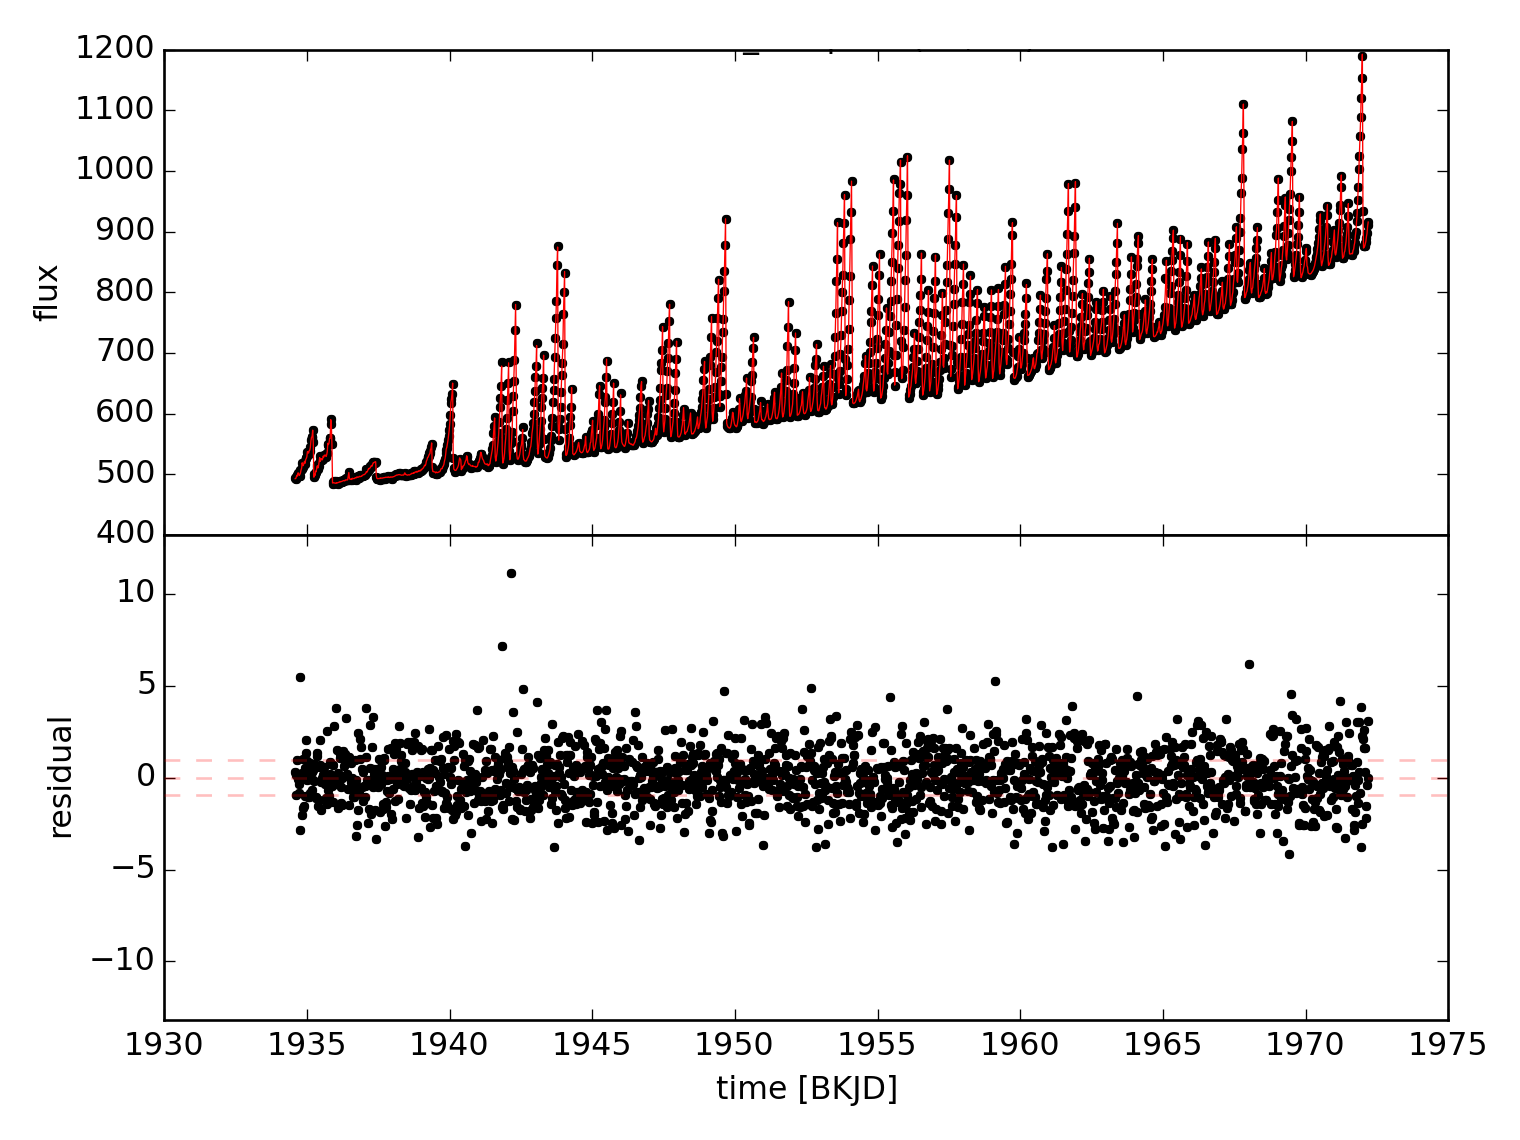
\includegraphics[width=0.95\textwidth]{f1a}
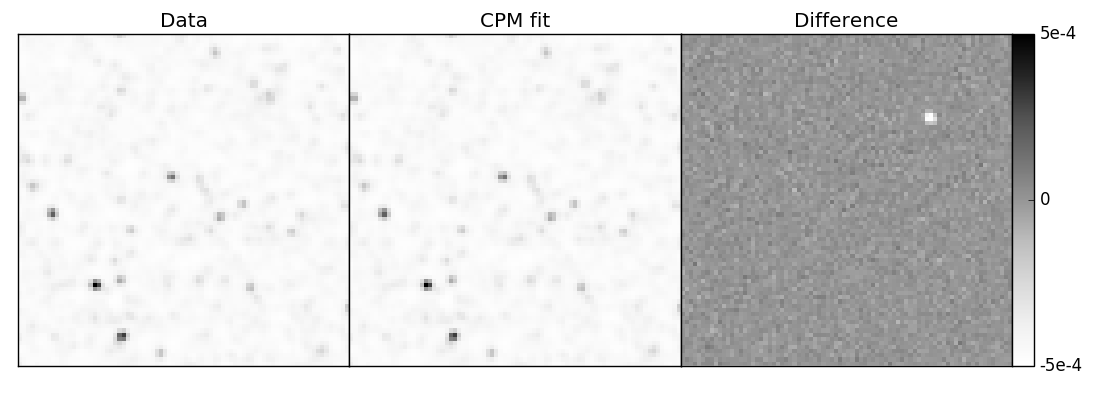
\includegraphics[width=0.95\textwidth]{f1b}
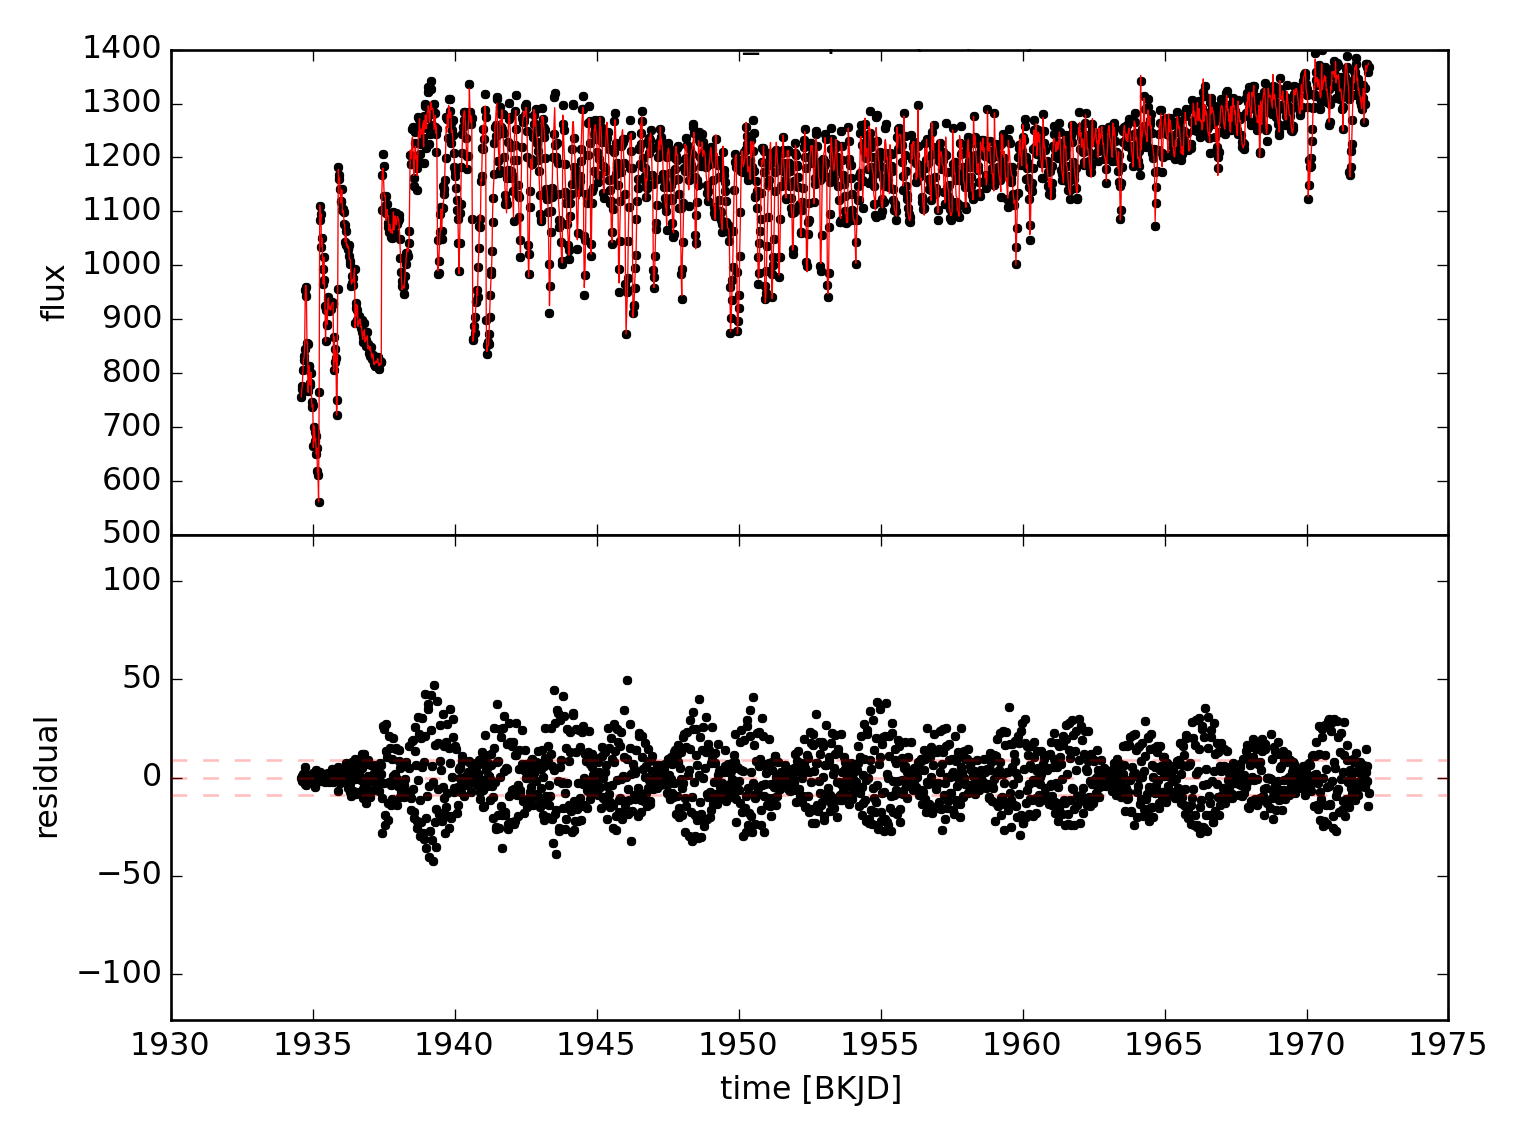
\includegraphics[width=0.95\textwidth]{f1c}
%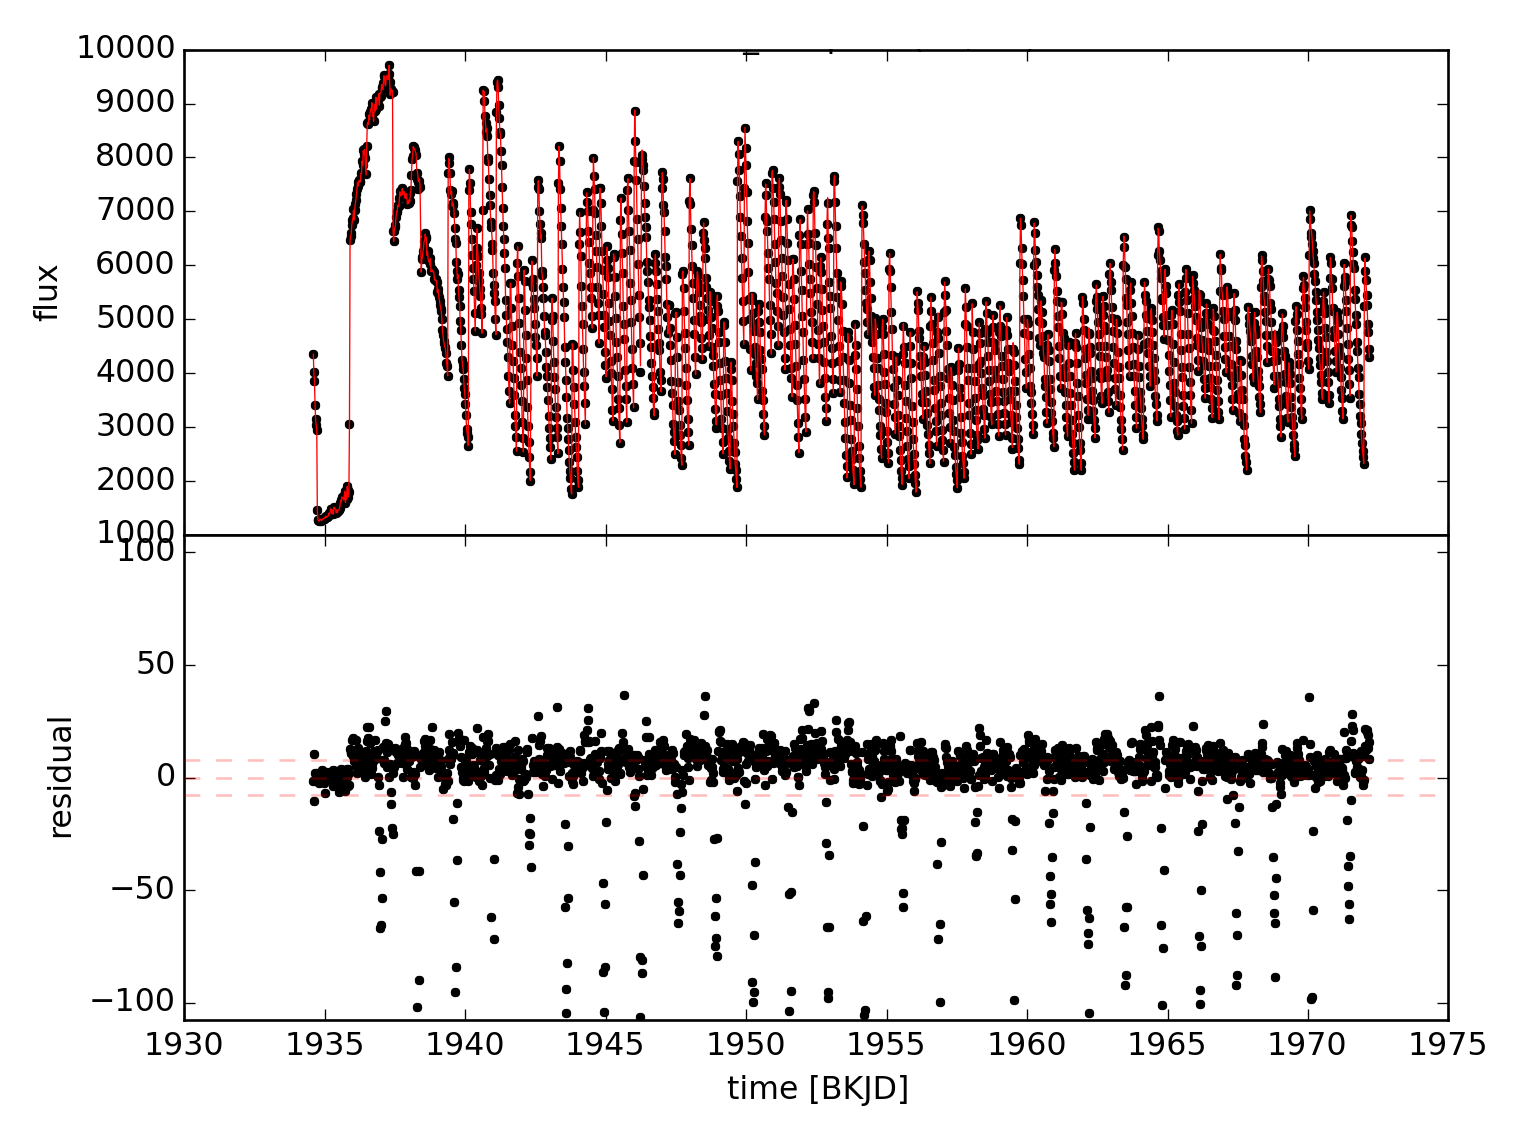
\includegraphics[width=0.95\textwidth]{f1d}
\end{center}
\caption{
\label{space}
  Mock Space-Based Data---an $80\times 80$ pixel mock data image patch with pointing motion and rotation variation. 
  From top to the bottom,  each row shows a snapshot from different times.
  \emph{Left:} mock data image;
  \emph{Middle:} the prediction of the \cpmdiff;
  \emph{Right:} the relative difference between the data and the prediction, the color bar shows the relative difference;
  the histogram shows the distribution of the difference and the dashed curve is the photon noise: Gaussian with $\sigma = 10^{-4}$.
  Note the small but significant astrometric shifts between images.
  Most of the difference-image pixel values are near zero, except for the variable source (upper-left corner), which shows that \cpmdiff\ can predict the image data, while detecting the variables. 
}
\end{figure}

\begin{figure}[p]
\begin{center}
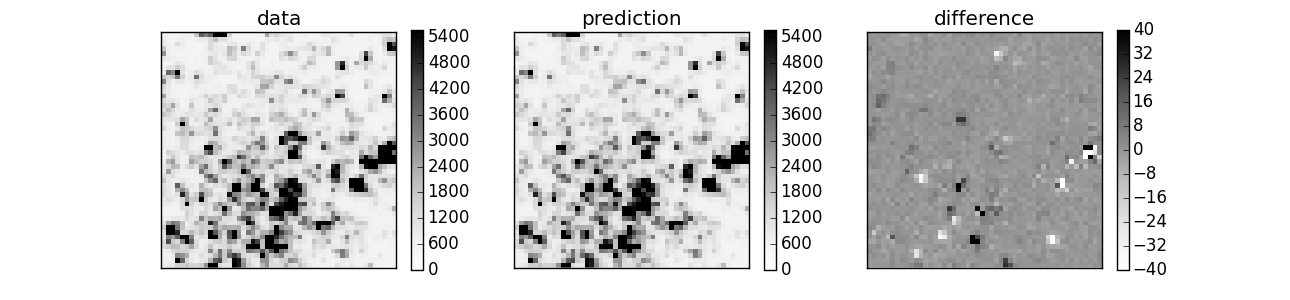
\includegraphics[width=0.95\textwidth]{f2a}
\end{center}
\caption{
\label{space_lc}
 The folded light curve of the variable star from the mock space-based data shown in Fig.~\ref{space}.
 The black points are the injected signal and the grey points are the recovered light curve from the \cpmdiff\ by co-adding the pixels in a $7\times 7$ patch around the source star.
}
\end{figure}

\subsection{Mock ground-based data}
In ground-based observations, in addition to changes in pointing and rotation, weather changes and atmospheric distortions will also affect the PSF. 
Therefore PSF variation was also included in the mock ground-based data. 
The pointing motion and rotation of the mock data are same as in the space-based test.
Variation of the PSF is achieved by varying the parameters $f_x, f_y, \phi$ defined in equation \ref{prf}.
Both $f_x$ and $f_y$ are drawn from uniform distribution ${\mathcal {U}}(2,3)$ pixels to restrict the full width half maximum of the PRF in both direction within 2-3 pixels and $\phi$ is drawn from ${\mathcal {U}}(0,\pi)$, which allows the orientation of the PRF to be in any direction.
Fig.~\ref{ground} and Fig.~\ref{ground_lc} show the same mock data and light curves as in space-based test, but with PRF variation included.  
As in the space-based test, the \cpmdiff\ was able to model both pointing motion and PRF variations, while still detecting the variable star in the differencing image.
Note that the PRF variations do degrade the quality of the difference image a little, since the changes of the PRF will change the correlation between pixels.
This experiment further confirms that \cpmdiff\ can calibrate both space-based and ground-based data.

\begin{figure}[p]
\begin{center}
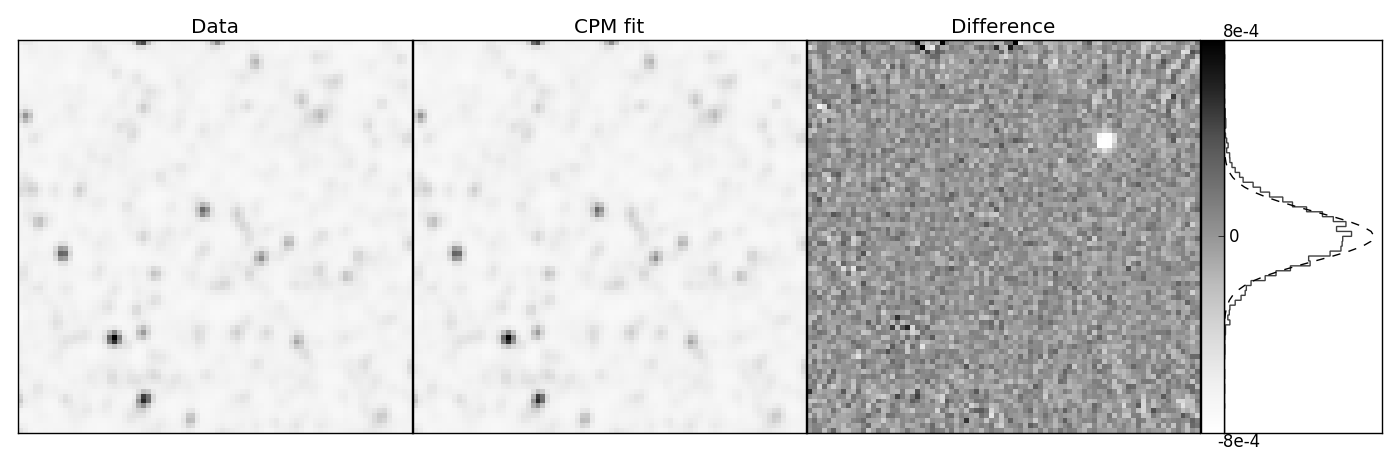
\includegraphics[width=0.95\textwidth]{f3a}
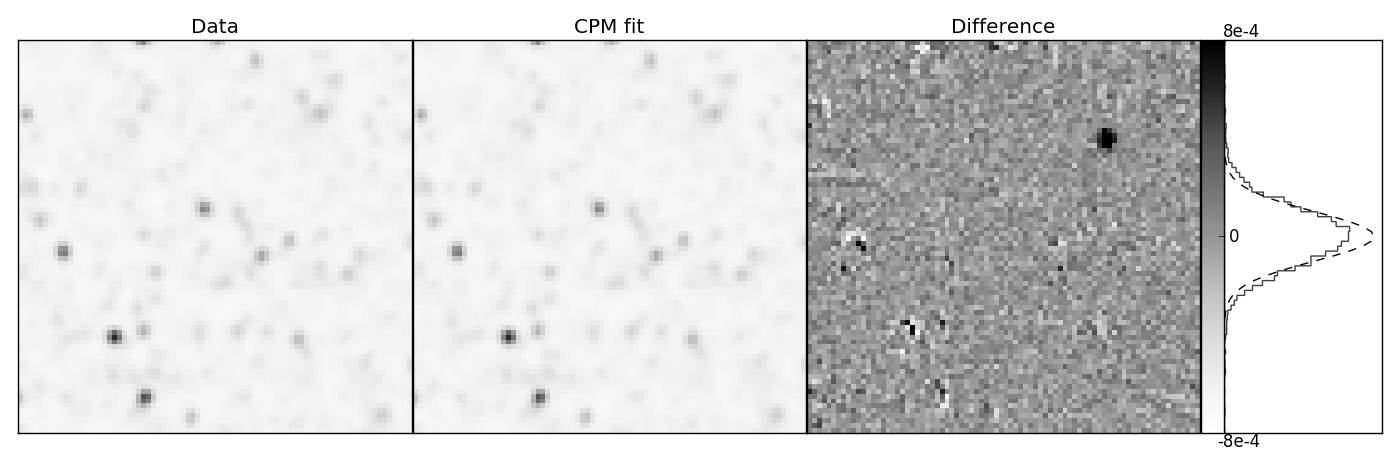
\includegraphics[width=0.95\textwidth]{f3b}
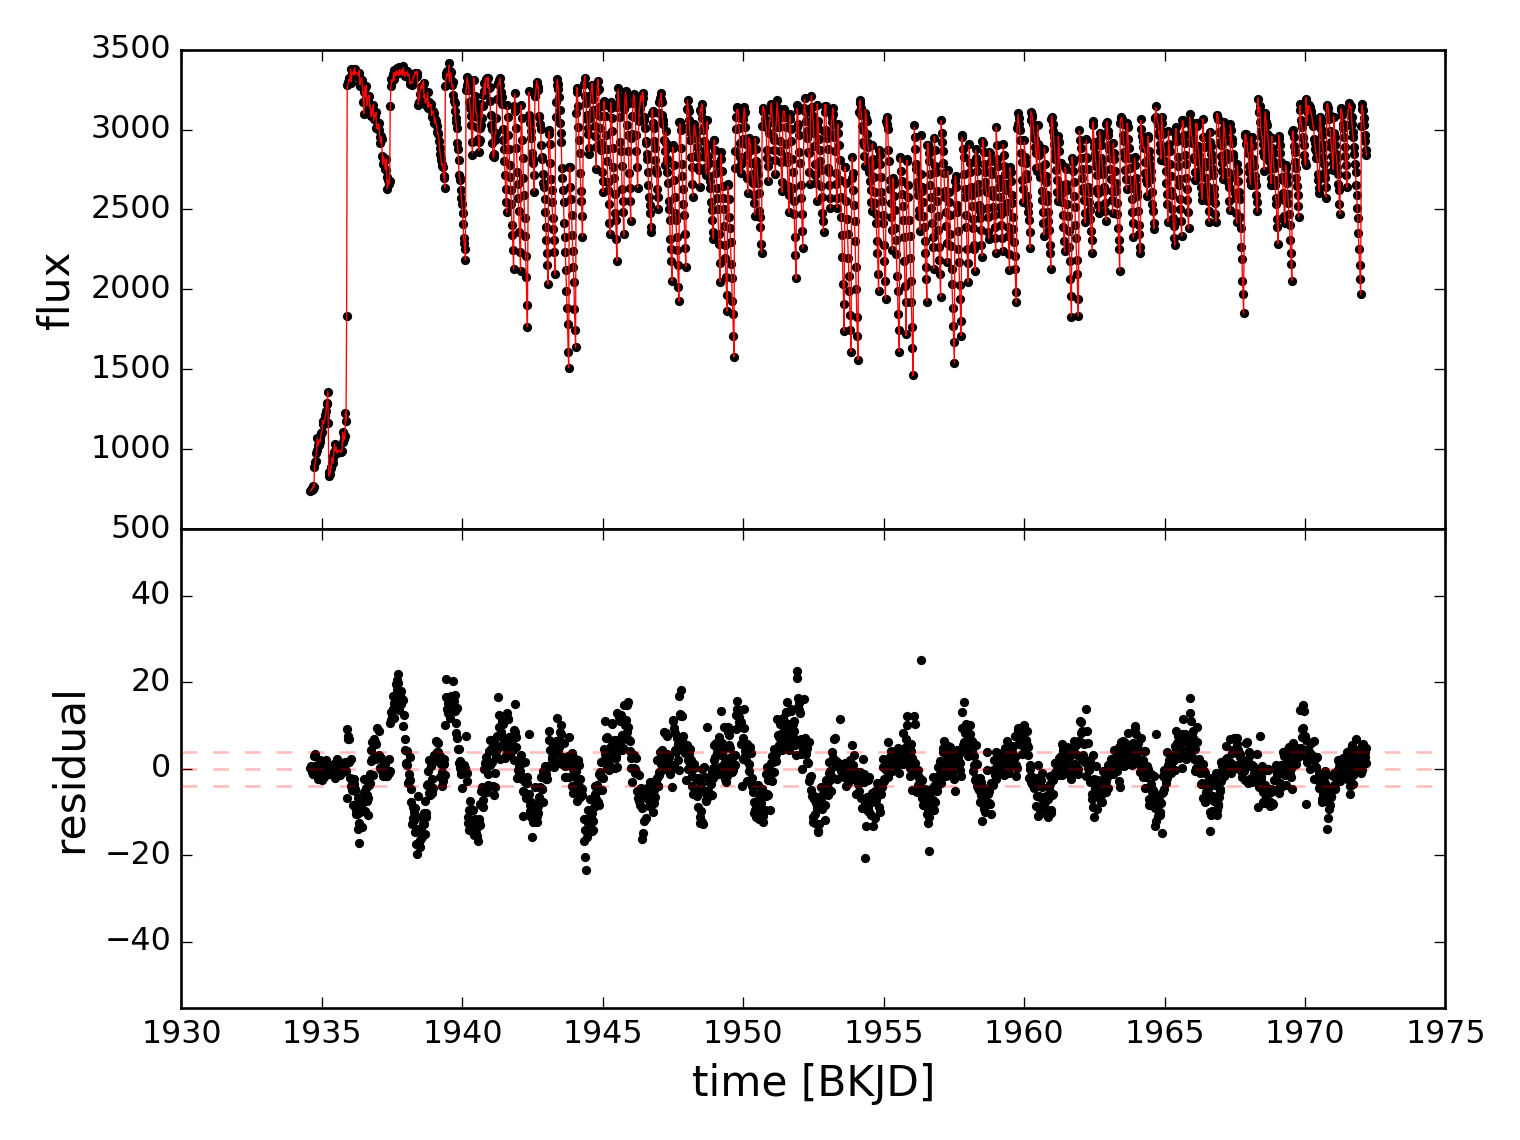
\includegraphics[width=0.95\textwidth]{f3c}
%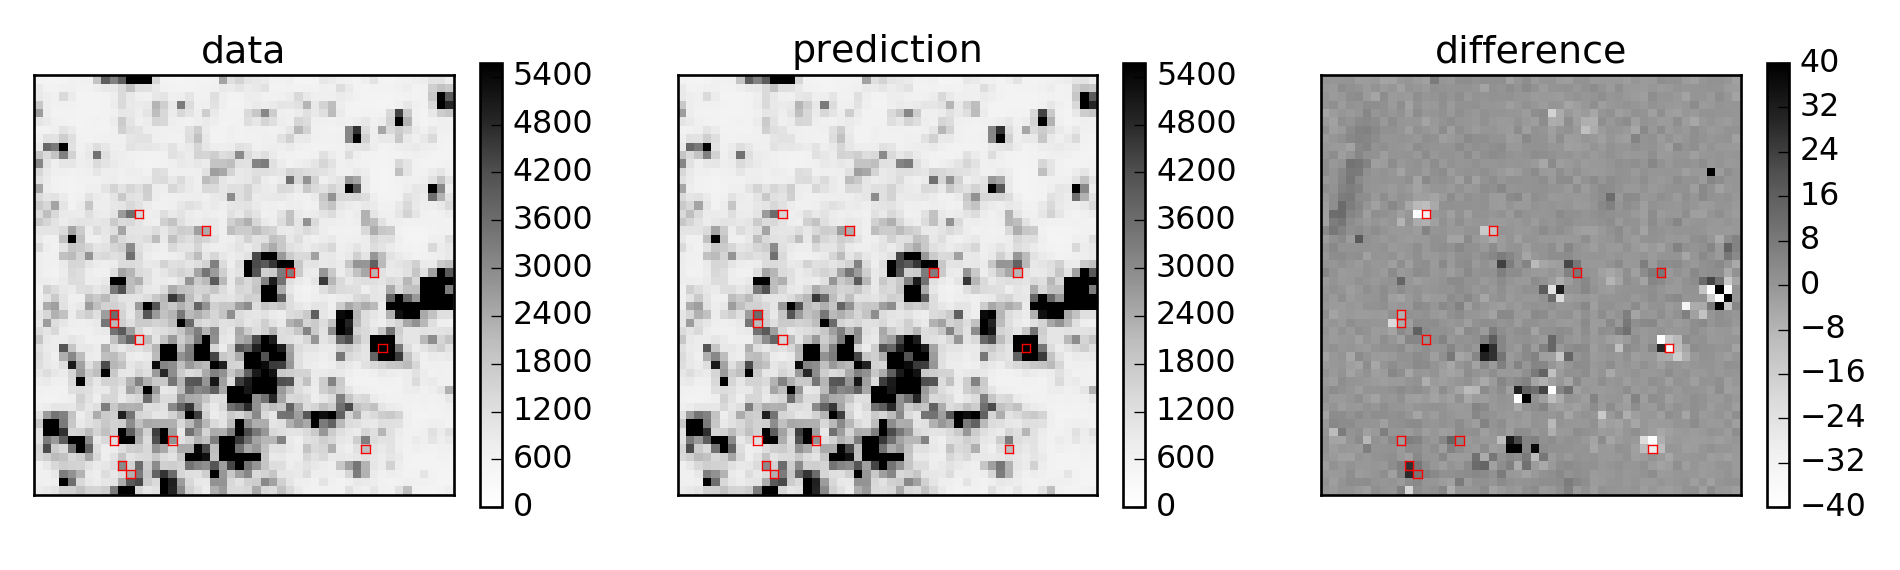
\includegraphics[width=0.95\textwidth]{f2d}
\end{center}
\caption{
  \label{ground}
  Mock Ground-Based Data---an $80\times 80$ pixel mock data image patch with pointing motion, rotation and PRF variation. 
  From top to the bottom,  each row shows a snapshot from different times.
  \emph{Left:} mock data image;
  \emph{Middle:} the prediction of the \cpmdiff;
  \emph{Right:} the relative difference between the data and the prediction, the color bar shows the relative difference; 
  the histogram shows the distribution of the difference and the dashed curve is the photon noise: Gaussian with $\sigma = 10^{-4}$. 
  As in the space-based test, \cpmdiff\ subtratcted all the constant stars and retained the variable sources with the mock ground-based data, which shows that the method can handle pointing motion, rotation and PRF variation altogether. 
}
\end{figure}

\begin{figure}[p]
\begin{center}
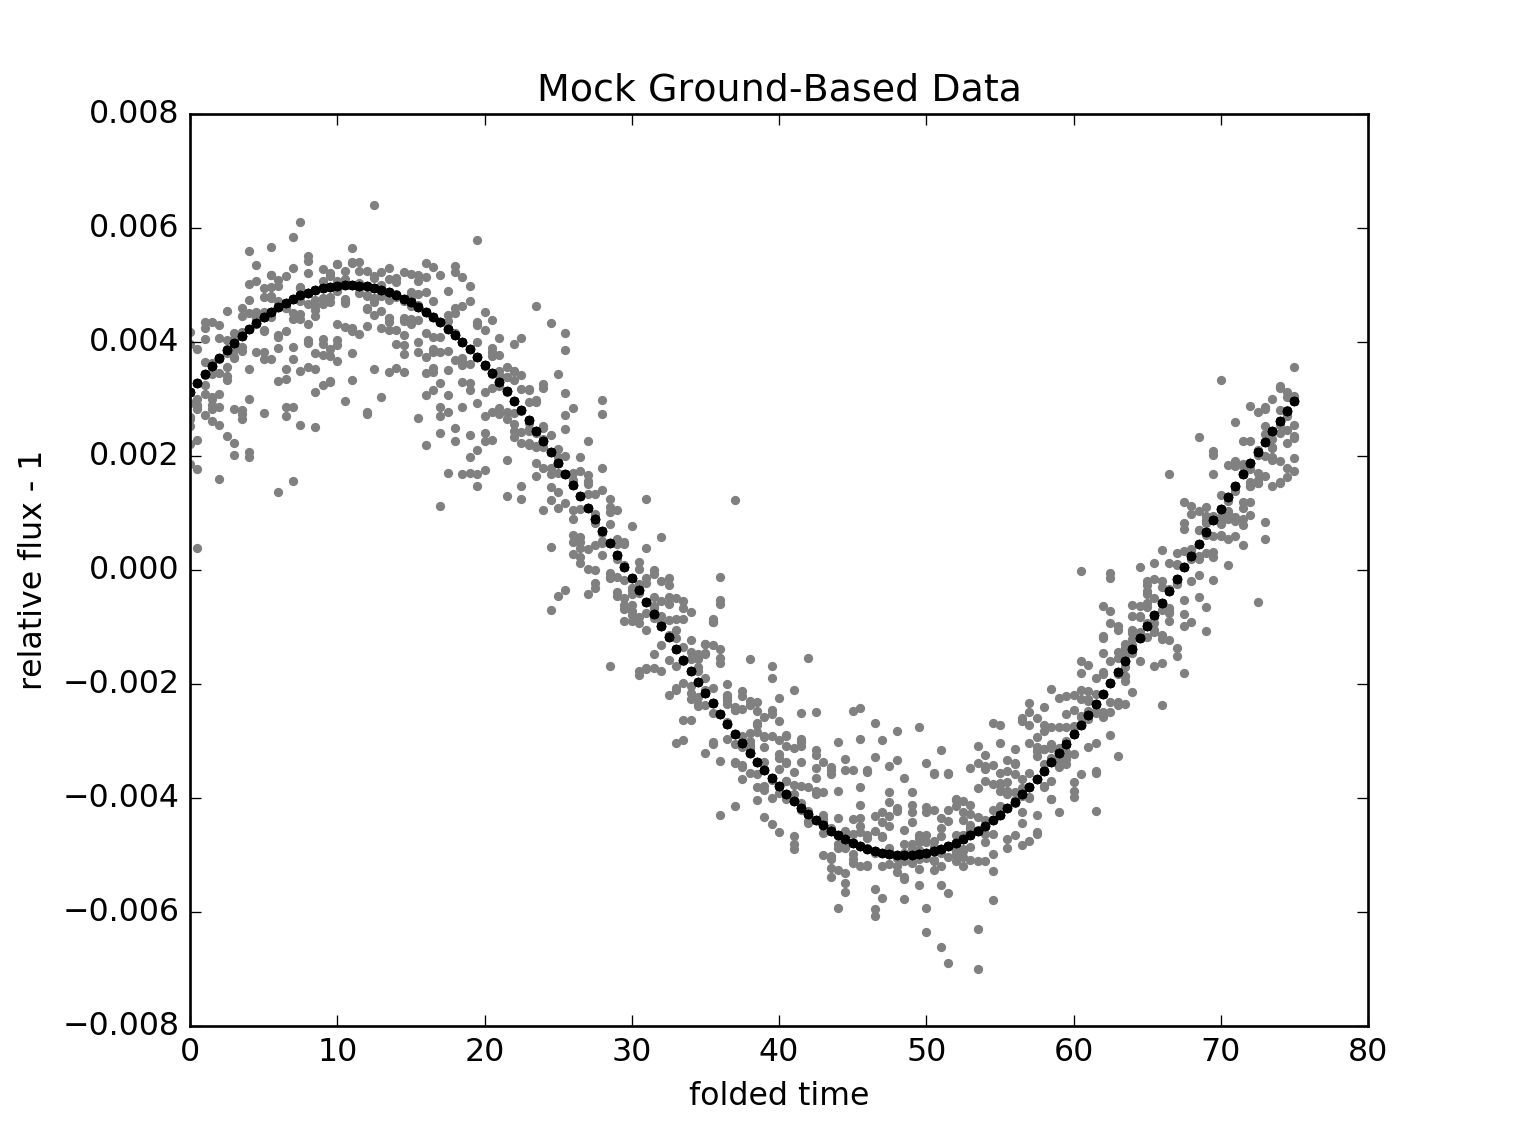
\includegraphics[width=0.95\textwidth]{f4a}
\end{center}
\caption{
\label{ground_lc}
 The folded light curve of the variable star from the mock ground-based data.
 The black points are the injected signal and the grey points are the recovered light curve from the \cpmdiff\ by co-adding the pixels in a $7\times 7$ patch around the source star.
}
\end{figure}

\subsection{\KTCN\ real data}
Now we test our method on a $64\times50$ pixel patch (\epic\ 200069960) from \KTCN\footnote{\url{https://keplerscience.arc.nasa.gov/k2-c9.html}}\citep{k2c9}, which was dedicated to a study of gravitational microlensing events.
This data set is an ideal test bed for difference imaging, since it observed a very crowded field near the bulge, where high precision photometry is difficult to achieve directly.
\cite{wei} has already applied \class\ on this data set and is able to model some microlensing events.

Fig.~\ref{k2c9} shows three snapshots of the data and the \cpmdiff\ of different times.
Constant sources in the dense field were almost all cancelled with the \cpm\ prediction, while variables (located at the white crosshairs) were preserved and can even be picked by eye from the difference image.
Variable sources were detected with the variation map (mean of absolute normalized deviations of the difference image). 
Light curves of six variable sources with highest signal to noise ratio is presented in Fig.~\ref{lightcurve} as examples. 
Each light curve was constructed with simple aperture photometry, by co-adding all the difference flux within a $3 \times 3$ aperture. 
Note that this is not optimal photometry; it is simply illustration of what is possible with this method.

\begin{figure}[p]
\begin{center}
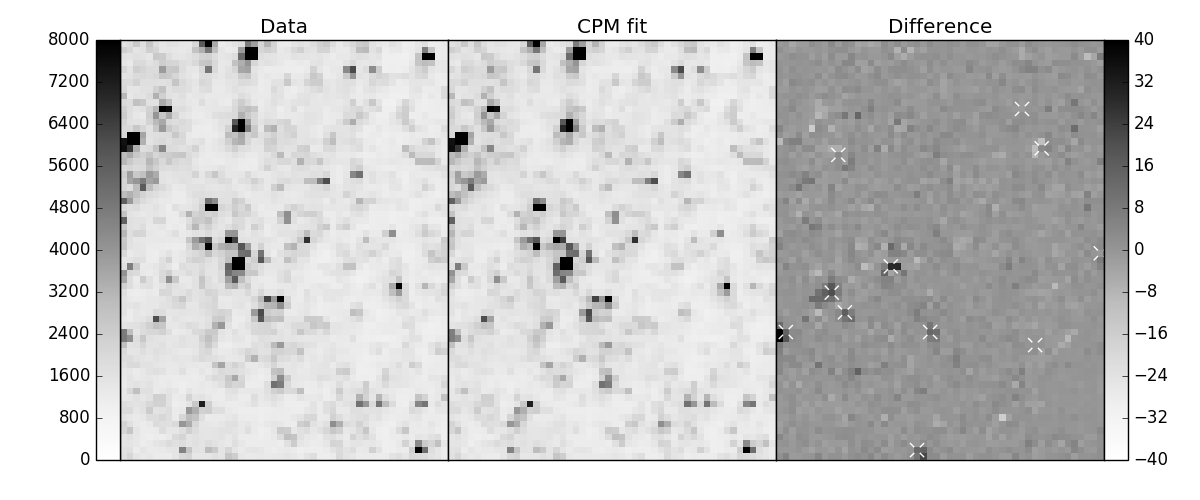
\includegraphics[width=0.95\textwidth]{f5a}
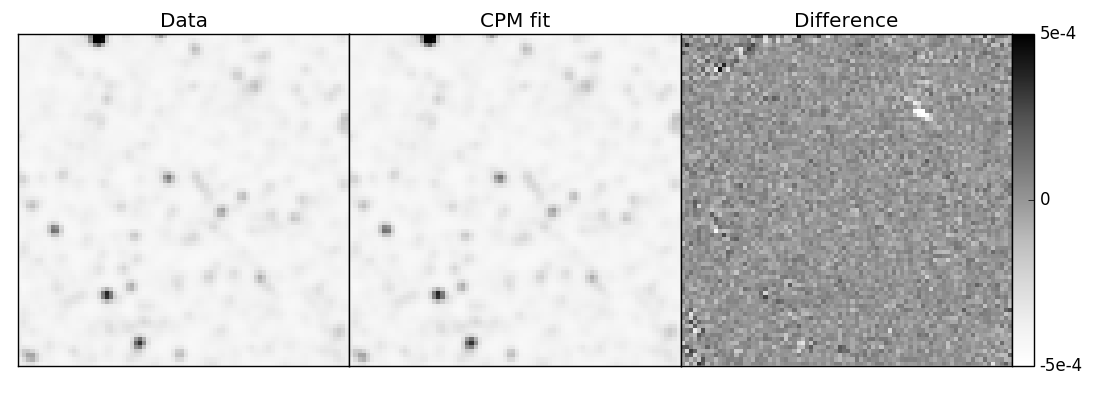
\includegraphics[width=0.95\textwidth]{f5b}
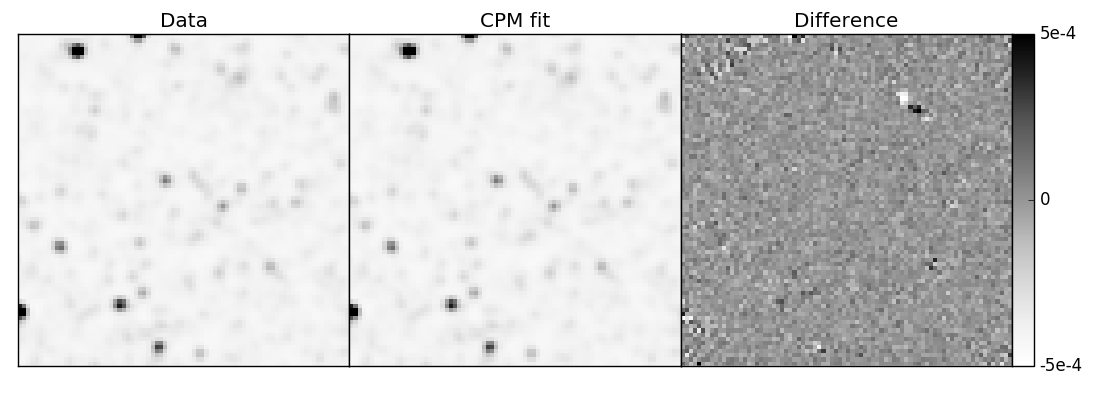
\includegraphics[width=0.95\textwidth]{f5c}
%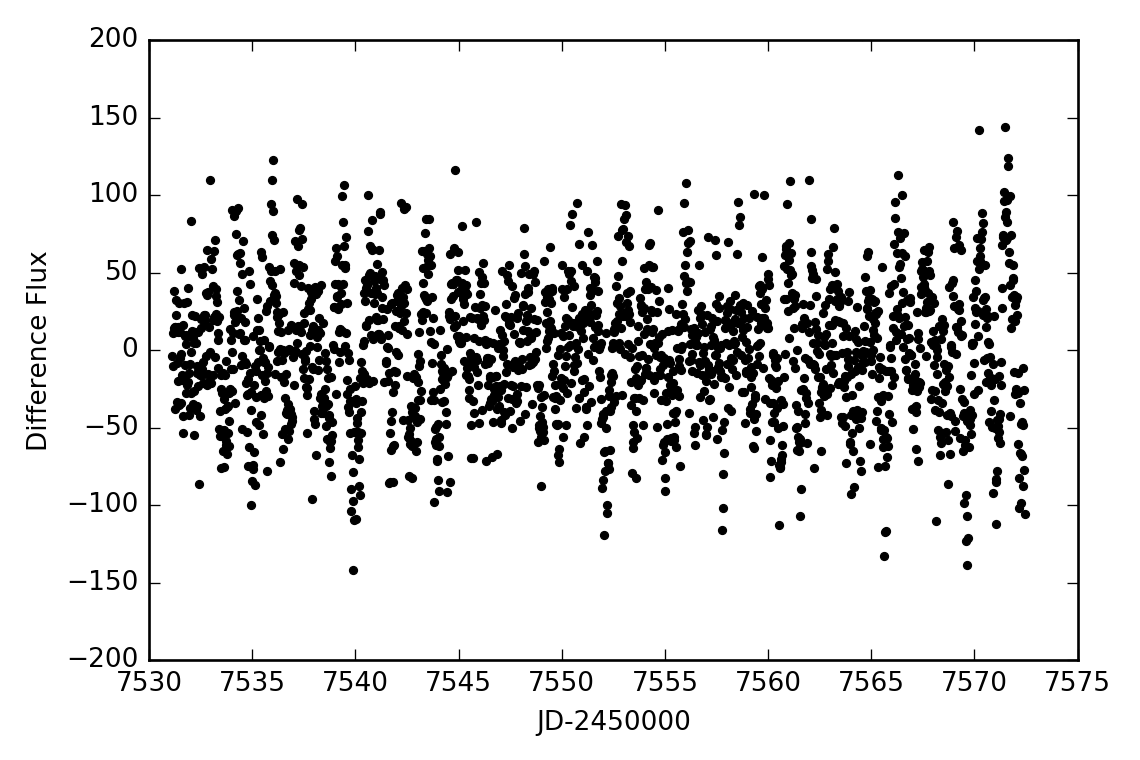
\includegraphics[width=0.95\textwidth]{f4d}
\end{center}
\caption{
  \label{k2c9}
  \KTCN\ Data---a $64\times 50$ pixel image patch from \KTCN\ (\epic\ 200069960). 
  From top to the bottom,  each row shows a snapshot from different times.
  \emph{Left:} data image;
  \emph{Middle:} the prediction of the \cpmdiff;
  \emph{Right:} the difference between the data and the prediction, white crosshairs indicate detected variable sources.
  The \cpmdiff\ subtracted all the constant sources in the data image, while preserve the variable sources in the difference image.
}
\end{figure}

\begin{figure}[p]
\begin{center}
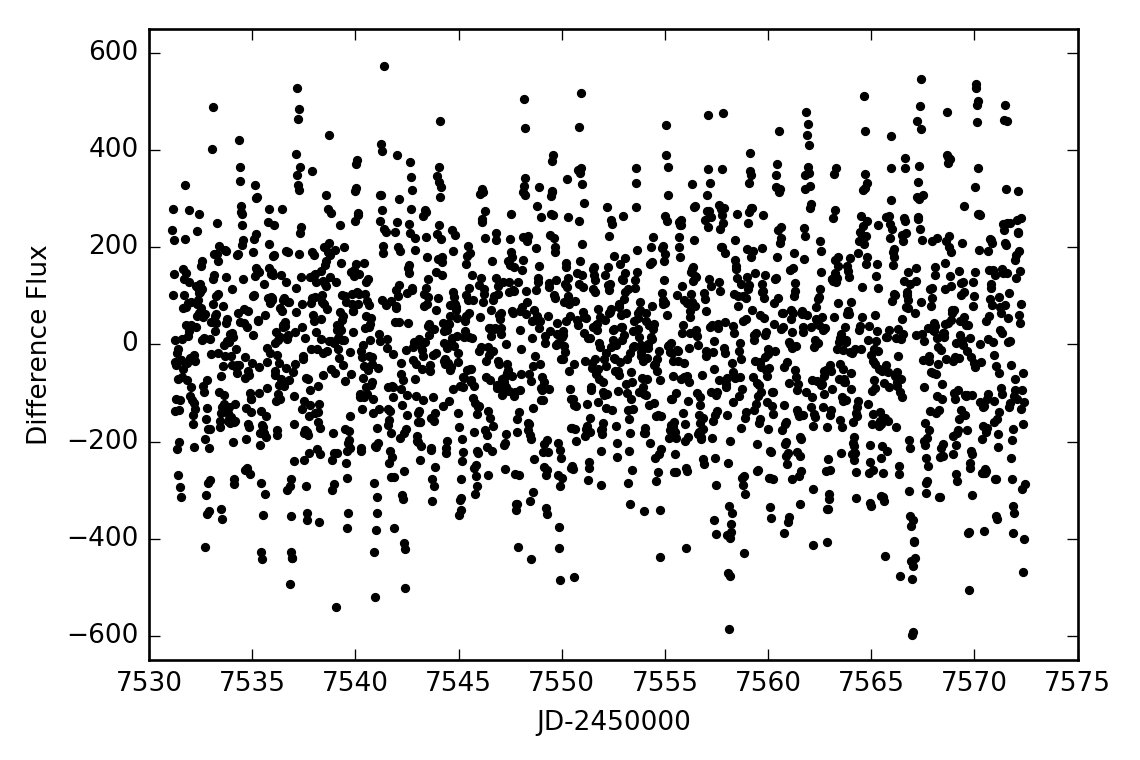
\includegraphics[width=0.48\textwidth]{f6a}
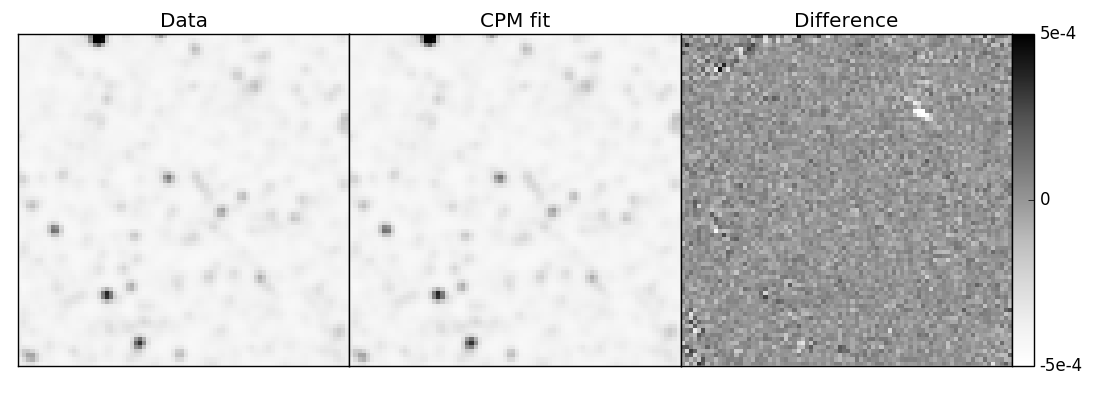
\includegraphics[width=0.48\textwidth]{f6b}
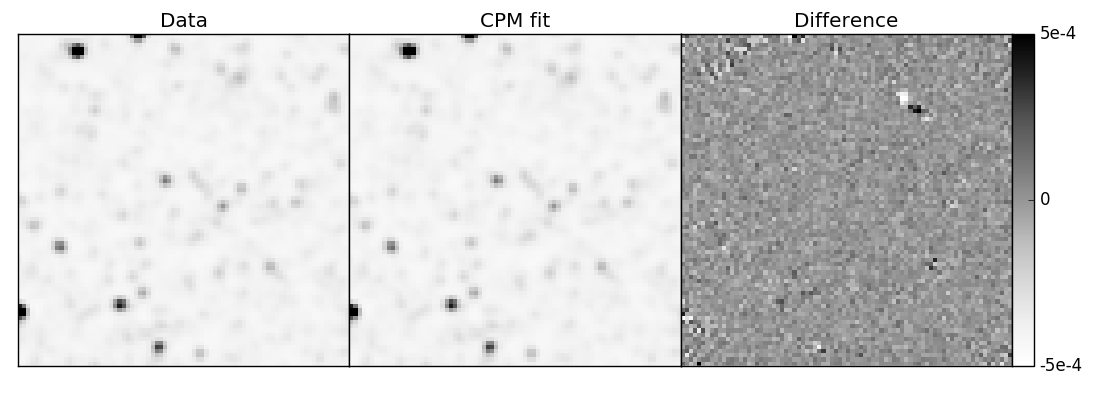
\includegraphics[width=0.48\textwidth]{f6c}
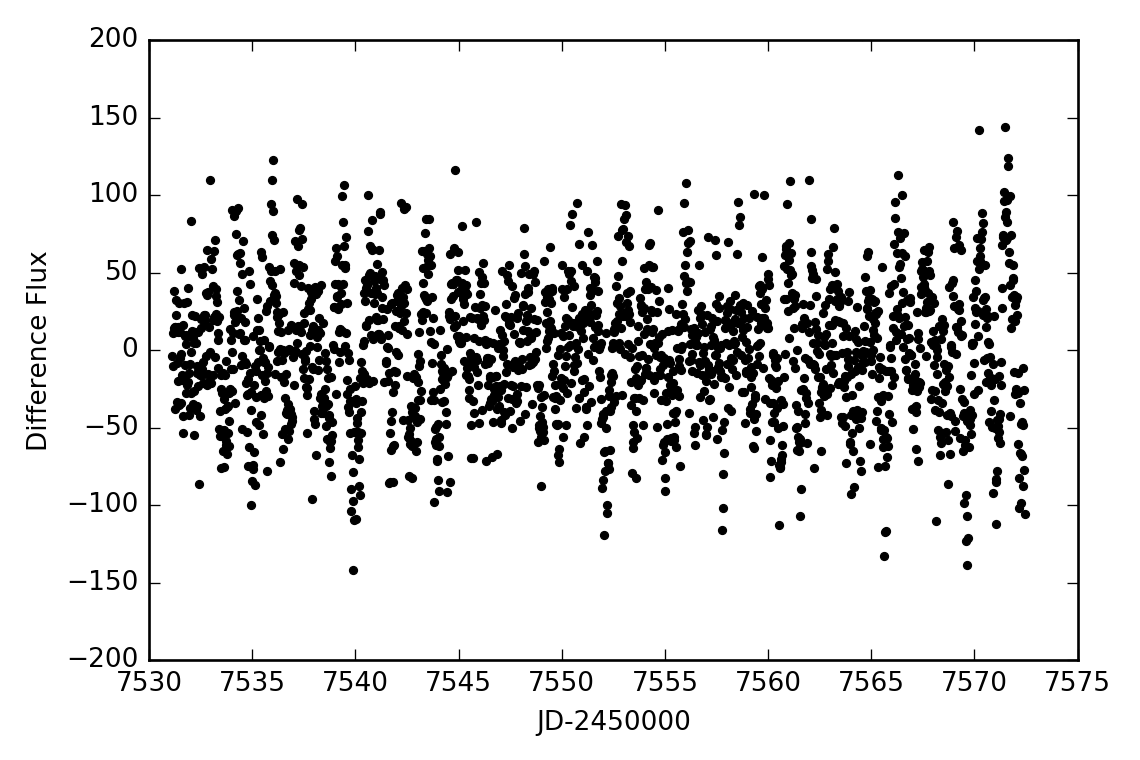
\includegraphics[width=0.48\textwidth]{f6d}
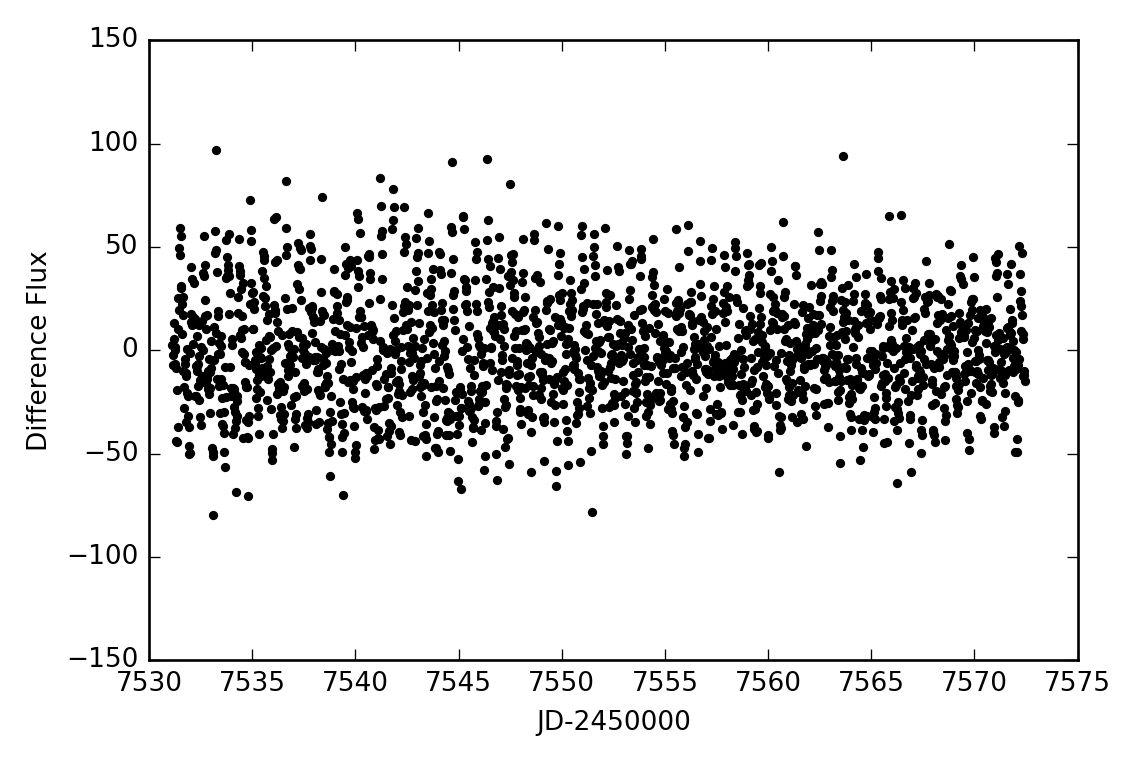
\includegraphics[width=0.48\textwidth]{f6e}
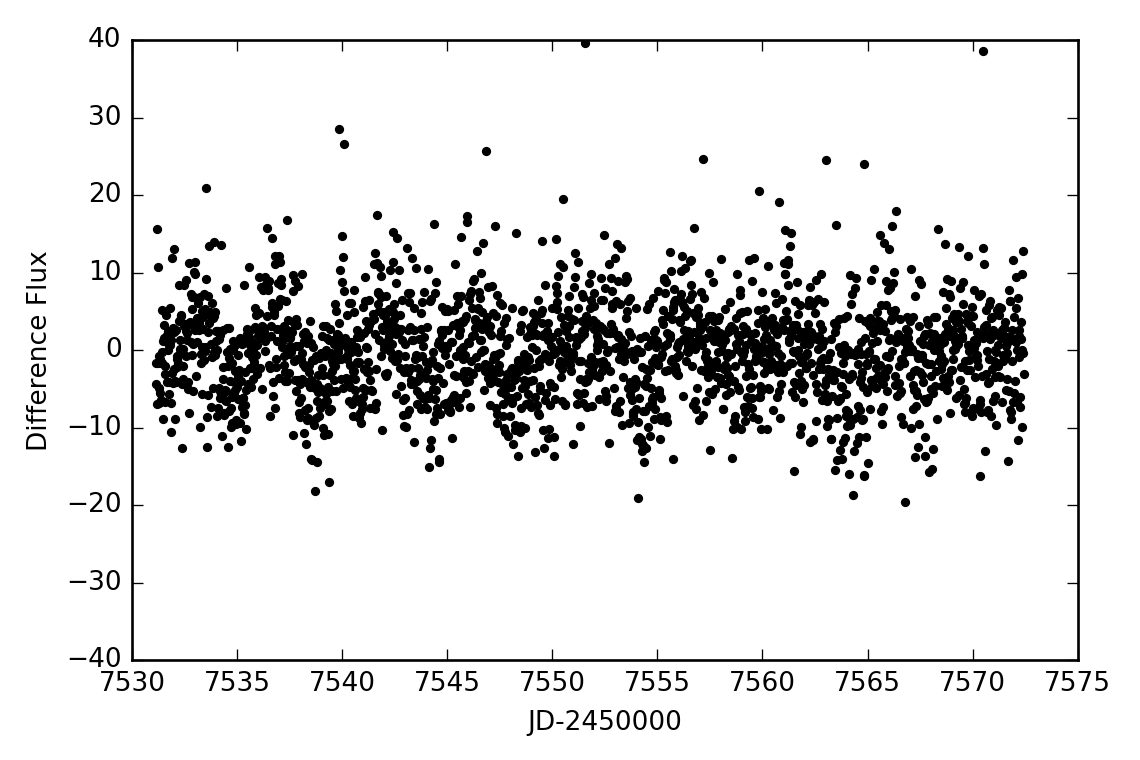
\includegraphics[width=0.48\textwidth]{f6f}
\end{center}
\caption{
  \label{lightcurve}
  \KTCN\ Data---six light curves extracted from \KTCN\ \epic\ 200069960 by \cpmdiff. 
  Each light curve was generated by co-adding all the difference flux within a $3\times 3$ aperature.
}
\end{figure}


\subsection{Limitation of \cpmdiff}\label{limits}
In previous sections,  \cpmdiff\ was proved on both mock and real data that the method is able to model pointing motion, rotation and PSF variations, with which variable sources detection and photometry can be achieved.
In this section, we want to push these variations to the limitation of \cpmdiff\ to define the scope of applicability of the method. Three experiments are conducted with large variations in pointing, roll and PSF.

First, mock data with the same rotation and PRF variations, but different amplitudes of pointing motion were tested by the model.
Here both $t_x$ and $t_y$ defined in equation \ref{transformation} were drawn from uniform distribution ${\mathcal {U}}(0,t_A)$ pixels, in which the upper limit $t_A$ defines the amplitude of the pointing motion.
Fig.~\ref{large_motion} shows that with the amplitude of the pointing motion increasing,  the quality of the difference image degrades dramatically, especially around relatively bright sources, because of the additional variabilities introduced by the motion of bright stars.
Similarly, in Fig.~\ref{large_rotation}, mock data with the same pointing and PRF variations, but different amplitudes of rotation were tested by the model.
In each data set, $\theta$ defined in equation \ref{transformation} was drawn from uniform distribution ${\mathcal {U}}(0,\theta_A)$ deg, in which the upper limit $\theta_A$ defines the amplitude of the rotation.
The corner of the difference image is much worse modelled, since the images are worse aligned in the corner due to the rotation. 
In order to quantitatively study the limitation of the pointing and rotation variation, the quality of each difference image is evaluated by the root-median-square residual (RMS residual) and the overall performance of the model is determined by the median of the RMS Residuals of all the difference images.
The amplitude of the pointing and rotation variations are both translated to the overall motions of stars in unit of FWHM of PRF.
Fig.~\ref{motion_rms} shows the median RMS residual as a function of the RMS motions of stars in different scenarios. 
These four lines in the plot show almost consistent relation that image quality degrades with moving stars by FWHMs.
This test also confirms the assumption that the registration should be good to about or better than one PSF width.
Finally, mock data with different amplitudes of PRF variation were tested.
Parameters $f_x$ and $f_y$ defined in equation \ref{prf} were drawn from uniform distribution ${\mathcal {U}}(2,f_{max})$ pixels, in which the width of the uniform distribution $f_{max}-2$ defines the amplitude of the PRF variation.
Fig.~\ref{large_prf} and Fig.~\ref{prf_rms} indicate that large PRF variations do degrade the performance of the model, since dramatic changes of the PRF can also largely change the correlation between pixels.
However, from the experiment, moderate PRF variations are still acceptable. 

\begin{figure}[p]
\begin{center}
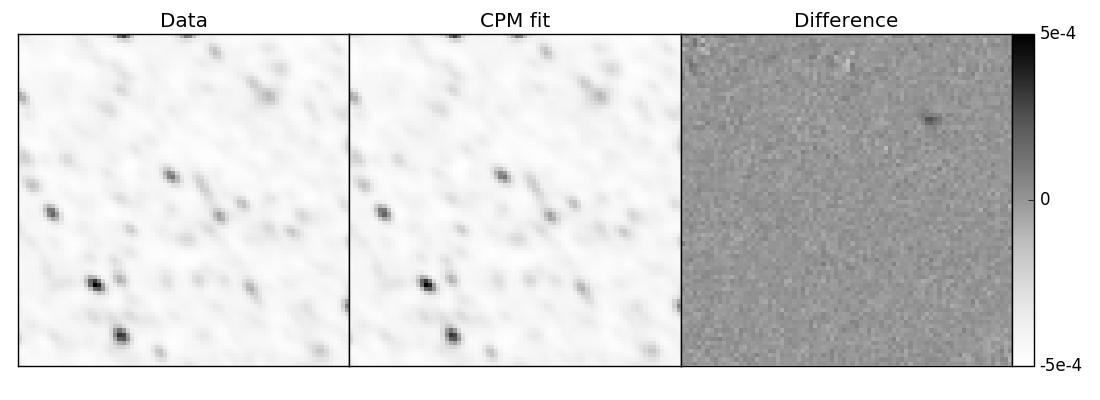
\includegraphics[width=0.95\textwidth]{f7a}
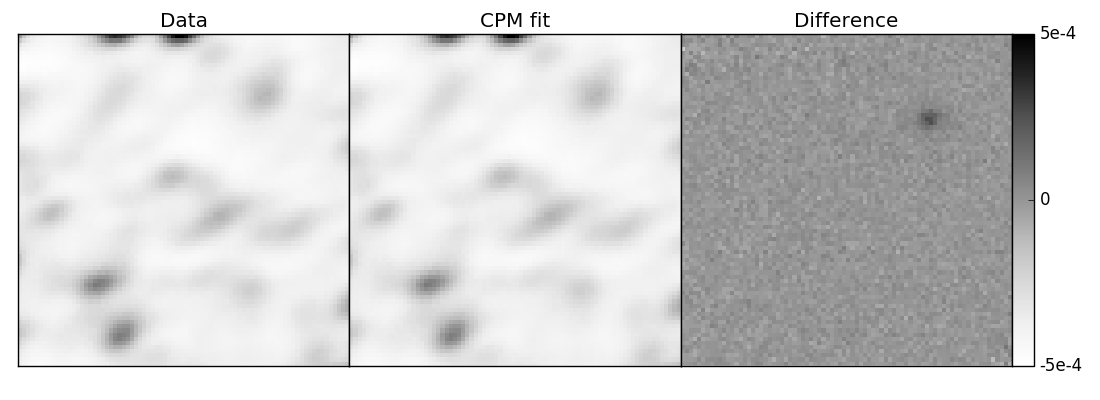
\includegraphics[width=0.95\textwidth]{f7b}
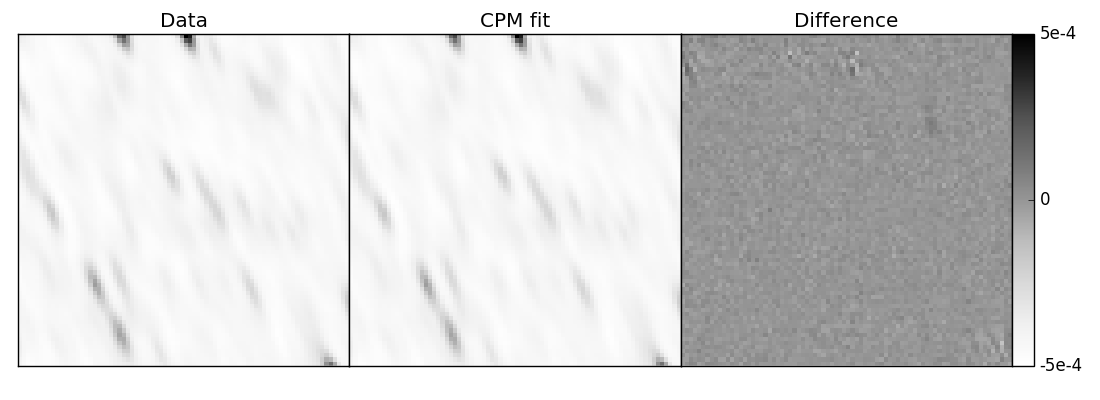
\includegraphics[width=0.95\textwidth]{f7c}
%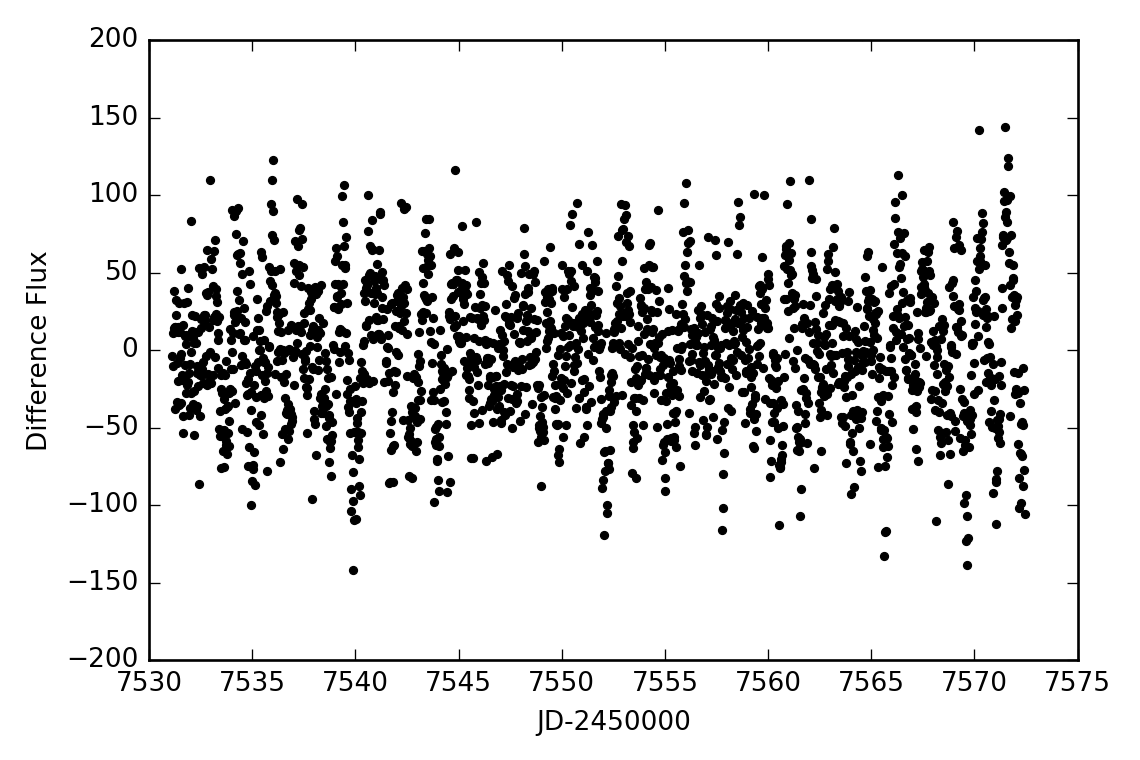
\includegraphics[width=0.95\textwidth]{f4d}
\end{center}
\caption{
  \label{large_motion}
  Three $80\times 80$ pixel mock data images with the same rotation and PSF variation, but different amplitudes of pointing motion. The amplitude of the pointing motion increases from top to the bottom.
  \emph{Left:} mock data image;
  \emph{Middle:} the prediction of the \cpmdiff;
  \emph{Right:} the relative difference between the data and the prediction, the color bar shows the relative difference; the histogram shows the distribution of the difference and the dashed curve is the photon noise: Gaussian with $\sigma = 10^{-4}$. 
  With the amplitude of the pointing motion increasing, the prediction of the \cpmdiff\ degrades.
}
\end{figure}

\begin{figure}[p]
\begin{center}
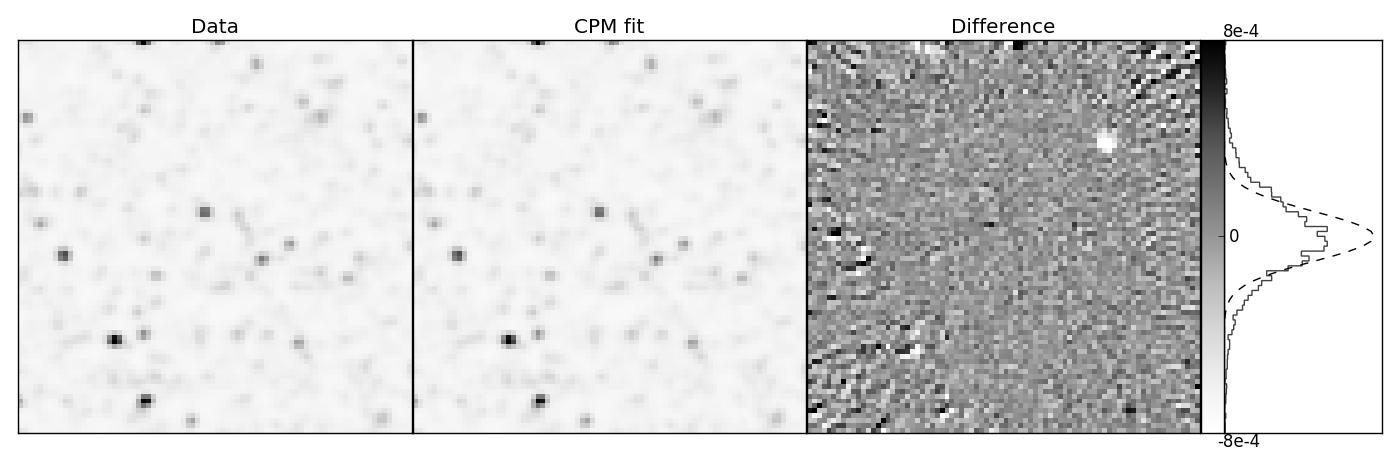
\includegraphics[width=0.95\textwidth]{f8a}
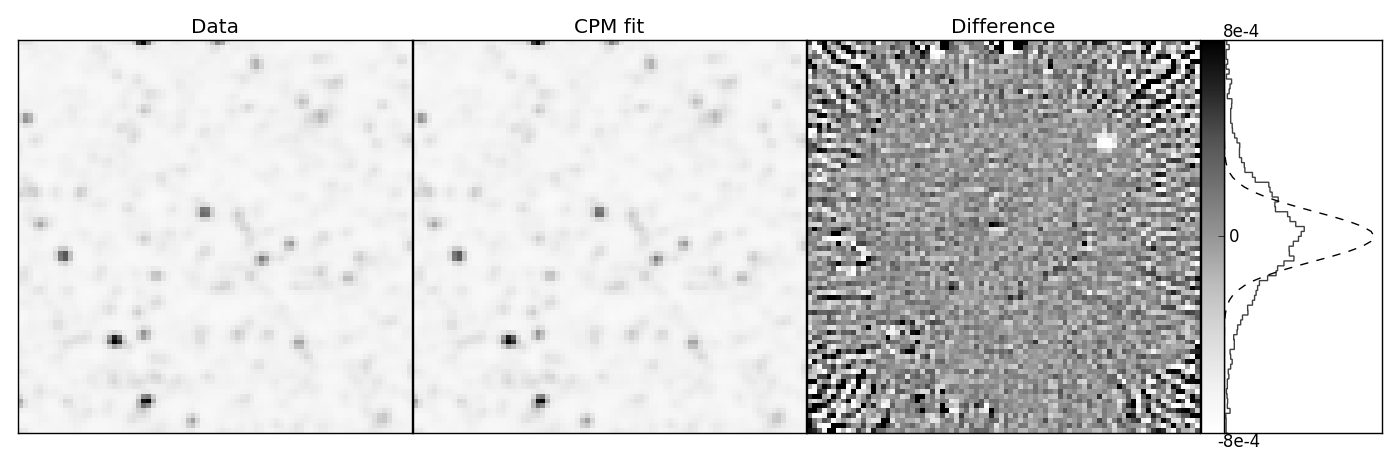
\includegraphics[width=0.95\textwidth]{f8b}
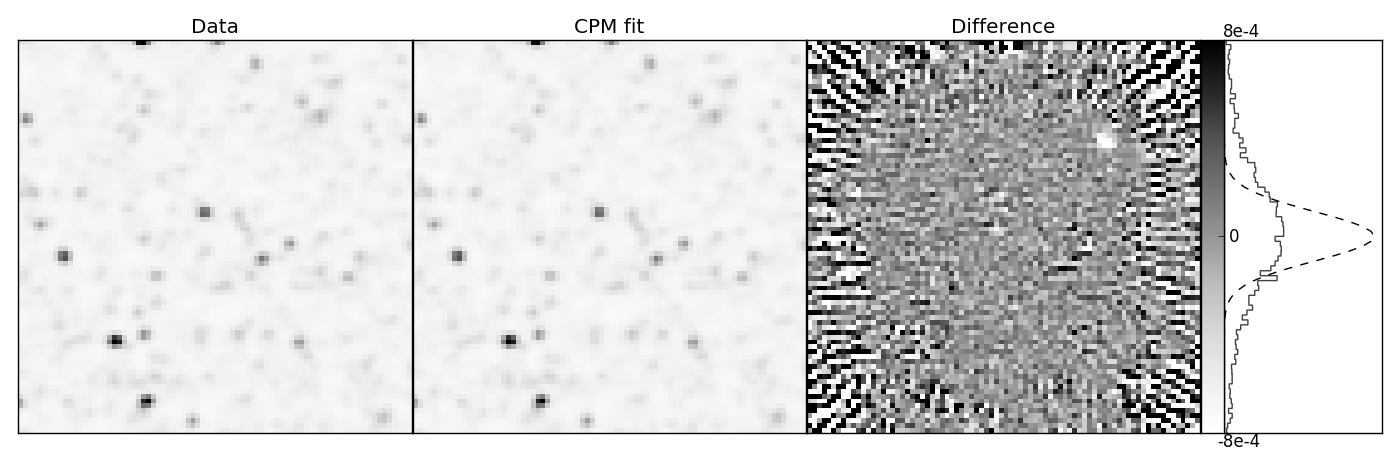
\includegraphics[width=0.95\textwidth]{f8c}
%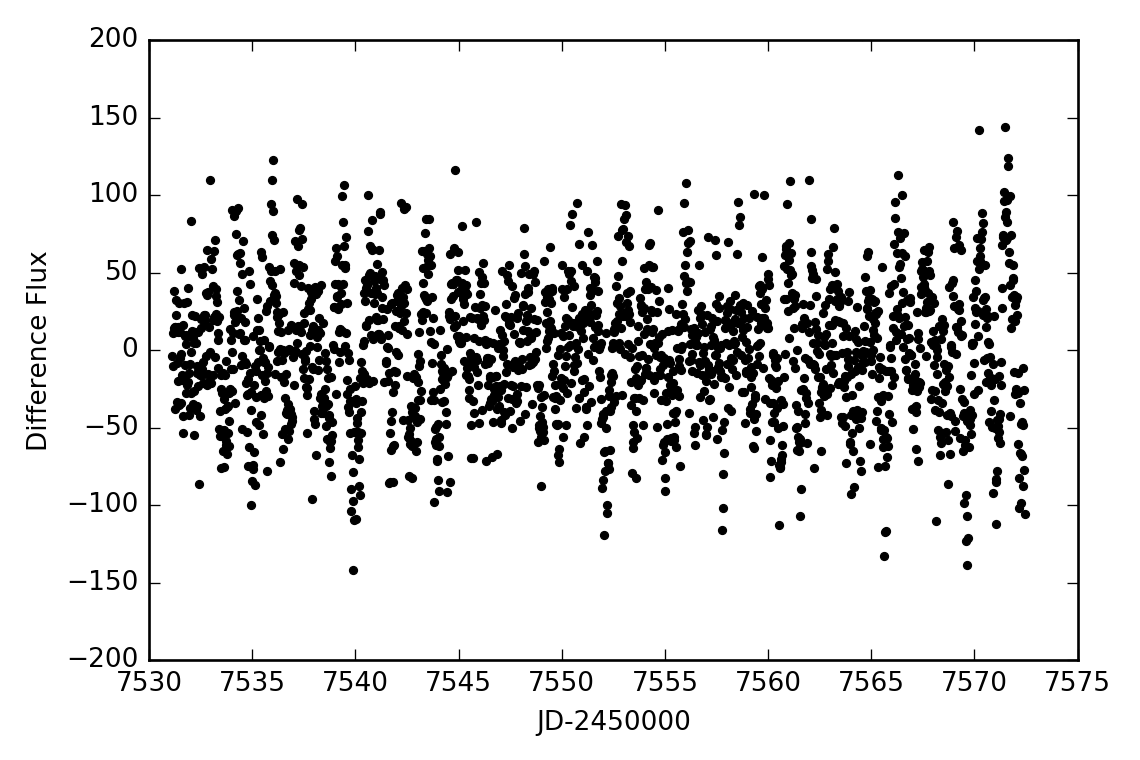
\includegraphics[width=0.95\textwidth]{f4d}
\end{center}
\caption{
  \label{large_rotation}
  Three $80\times 80$ pixel mock data images with the same pointing motion and PRF variation, but different amplitudes of rotation. The amplitude of rotation increases from top to the bottom.
  \emph{Left:} mock data image;
  \emph{Middle:} the prediction of the \cpmdiff;
  \emph{Right:} the relative difference between the data and the prediction, the color bar shows the relative difference; the histogram shows the distribution of the difference and the dashed curve is the photon noise: Gaussian with $\sigma = 10^{-4}$. 
  With the amplitude of rotation increasing, the quality of the difference image drops dramatically in the corner, while almostly remains unchanged in the middle.
}
\end{figure}

\begin{figure}[p]
\begin{center}
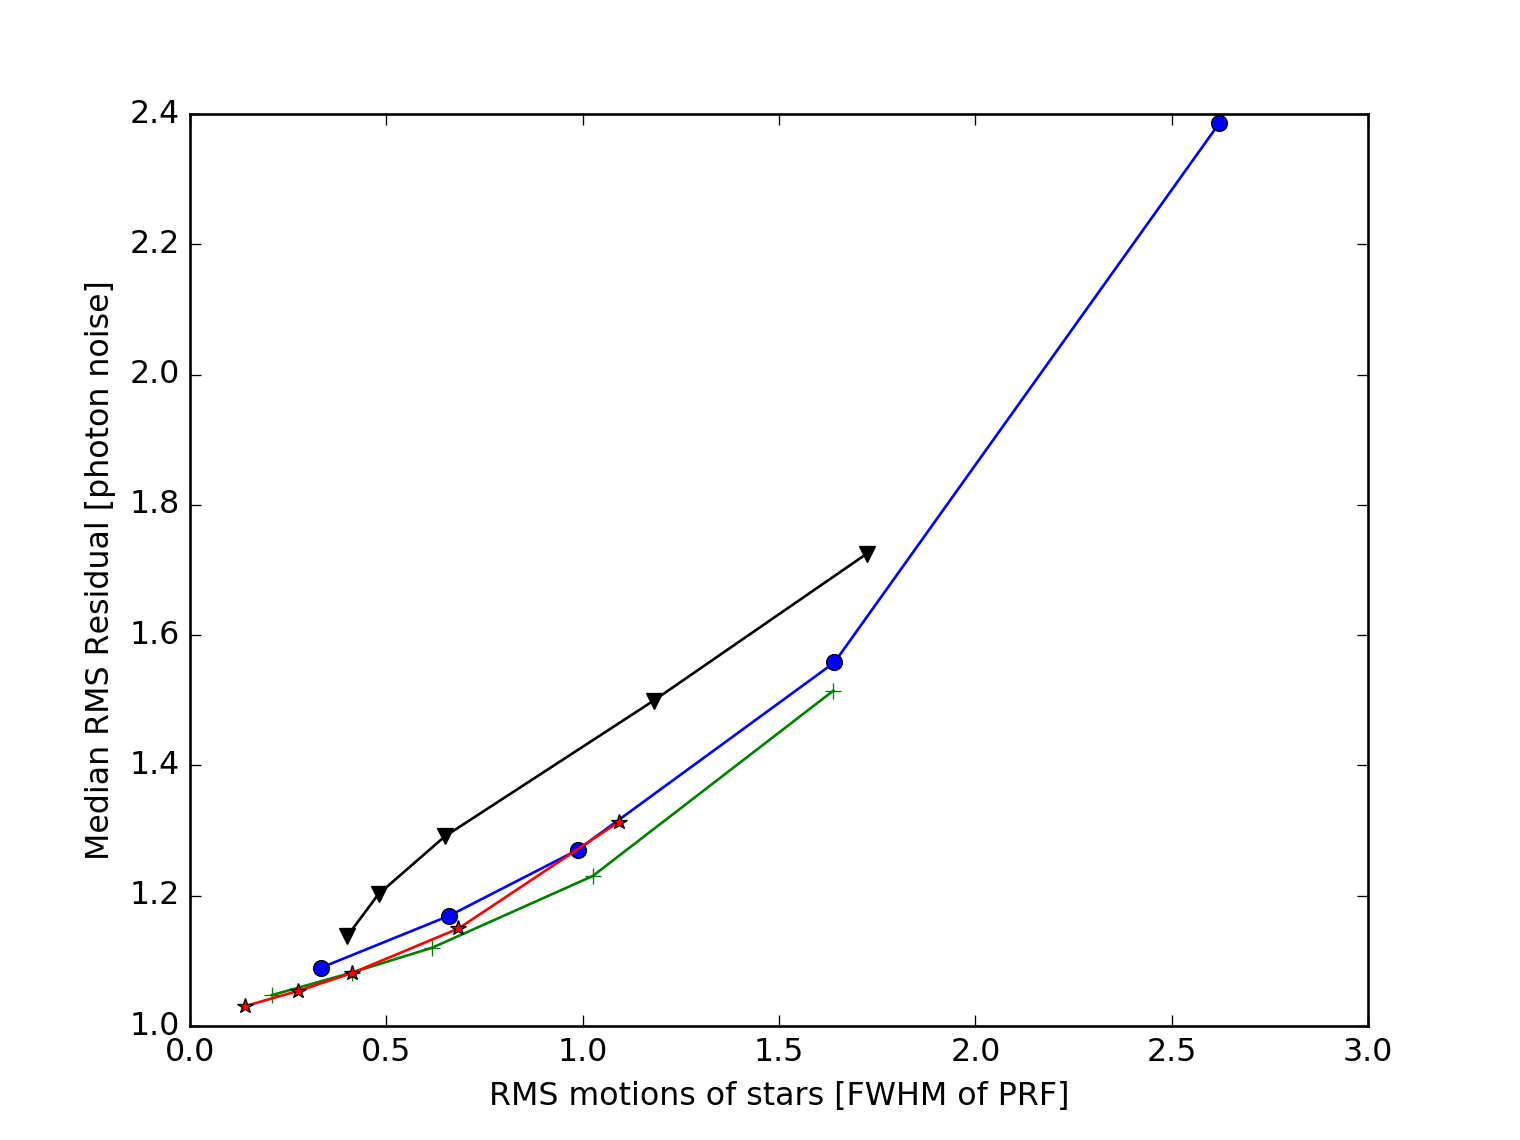
\includegraphics[width=0.95\textwidth]{move_new_p}
\end{center}
\caption{
\label{motion_rms}
 Median root-mean-square residual as a function of the root-mean-square motions of stars in unit of FWHM of PRF.
 Different markers and colors indicate different scenarios.
 \emph{Blue dots}: pointing variation with FWHM of PRF = 2.5 pixels;
 \emph{Green cross}: pointing variation with FWHM of PRF = 4 pixels;
 \emph{Red stars}: pointing variation with FWHM of PRF = 6 pixels;
 \emph{Black triangle}: rotation with FWHM of PRF = 2.5 pixels;
}
\end{figure}


\begin{figure}[p]
\begin{center}
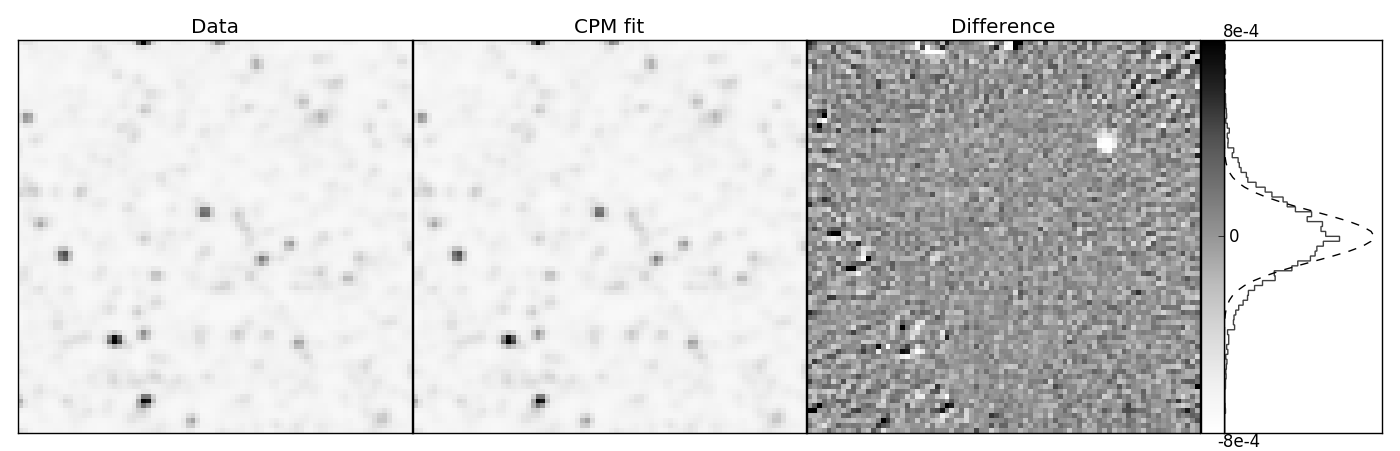
\includegraphics[width=0.95\textwidth]{f9a}
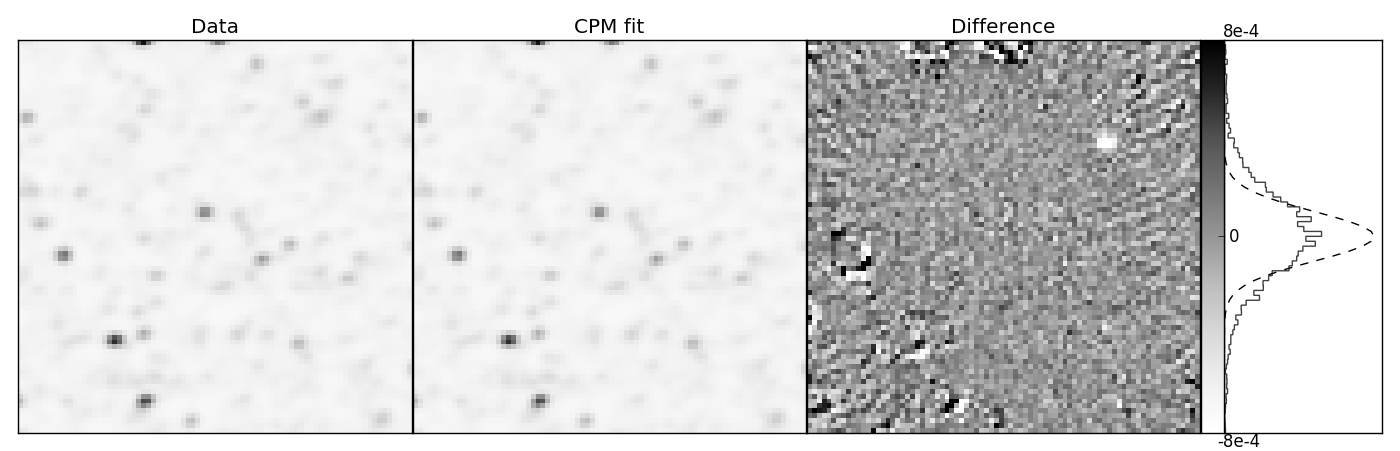
\includegraphics[width=0.95\textwidth]{f9b}
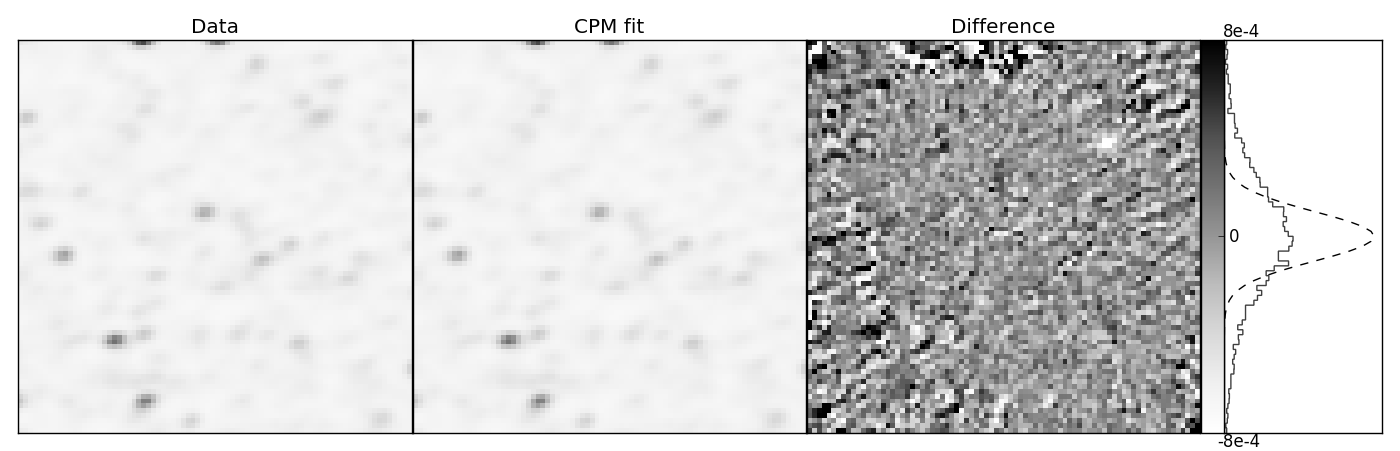
\includegraphics[width=0.95\textwidth]{f9c}
%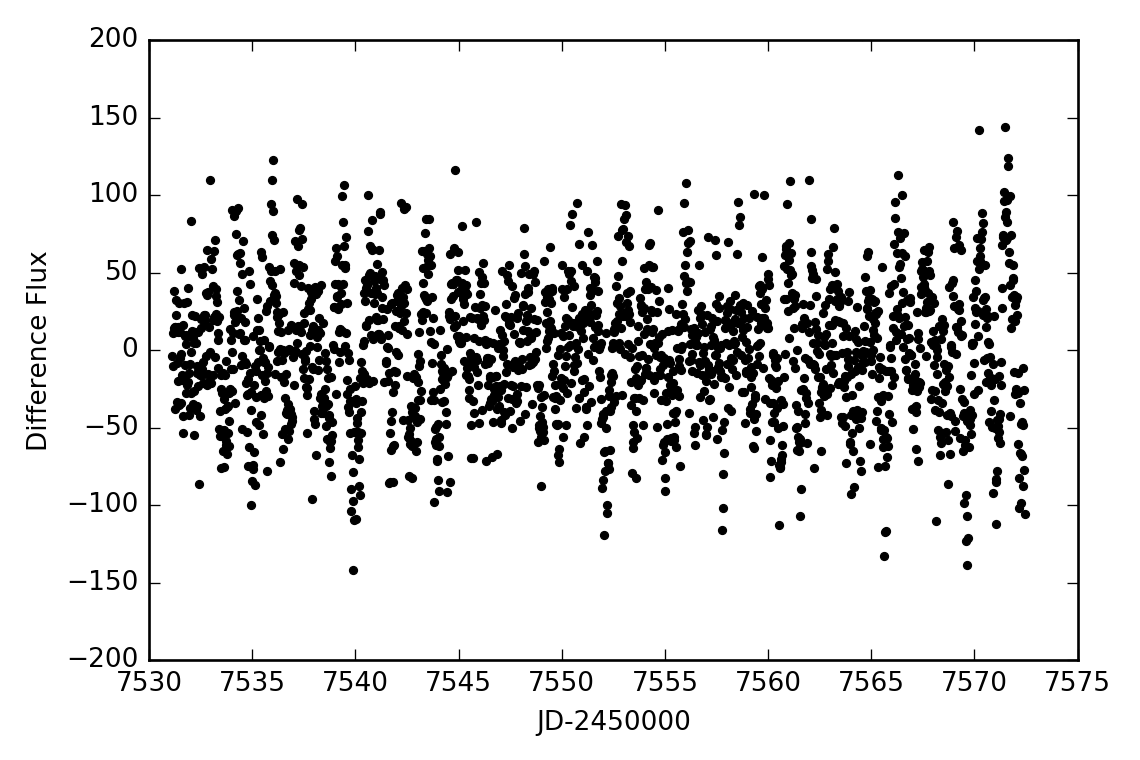
\includegraphics[width=0.95\textwidth]{f4d}
\end{center}
\caption{
  \label{large_prf}
  Three $80\times 80$ pixel mock data images with the same pointing motion and rotation, but different amplitudes of PRF variation. The amplitude of PRF variation increases from top to the bottom.
  \emph{Left:} mock data image;
  \emph{Middle:} the prediction of the \cpmdiff;
  \emph{Right:} the relative difference between the data and the prediction, the color bar shows the relative difference; the histogram shows the distribution of the difference and the dashed curve is the photon noise: Gaussian with $\sigma = 10^{-4}$. 
  With the amplitude of PRF variation increasing, the quality of the difference image degrades.
}
\end{figure}

\begin{figure}[p]
\begin{center}
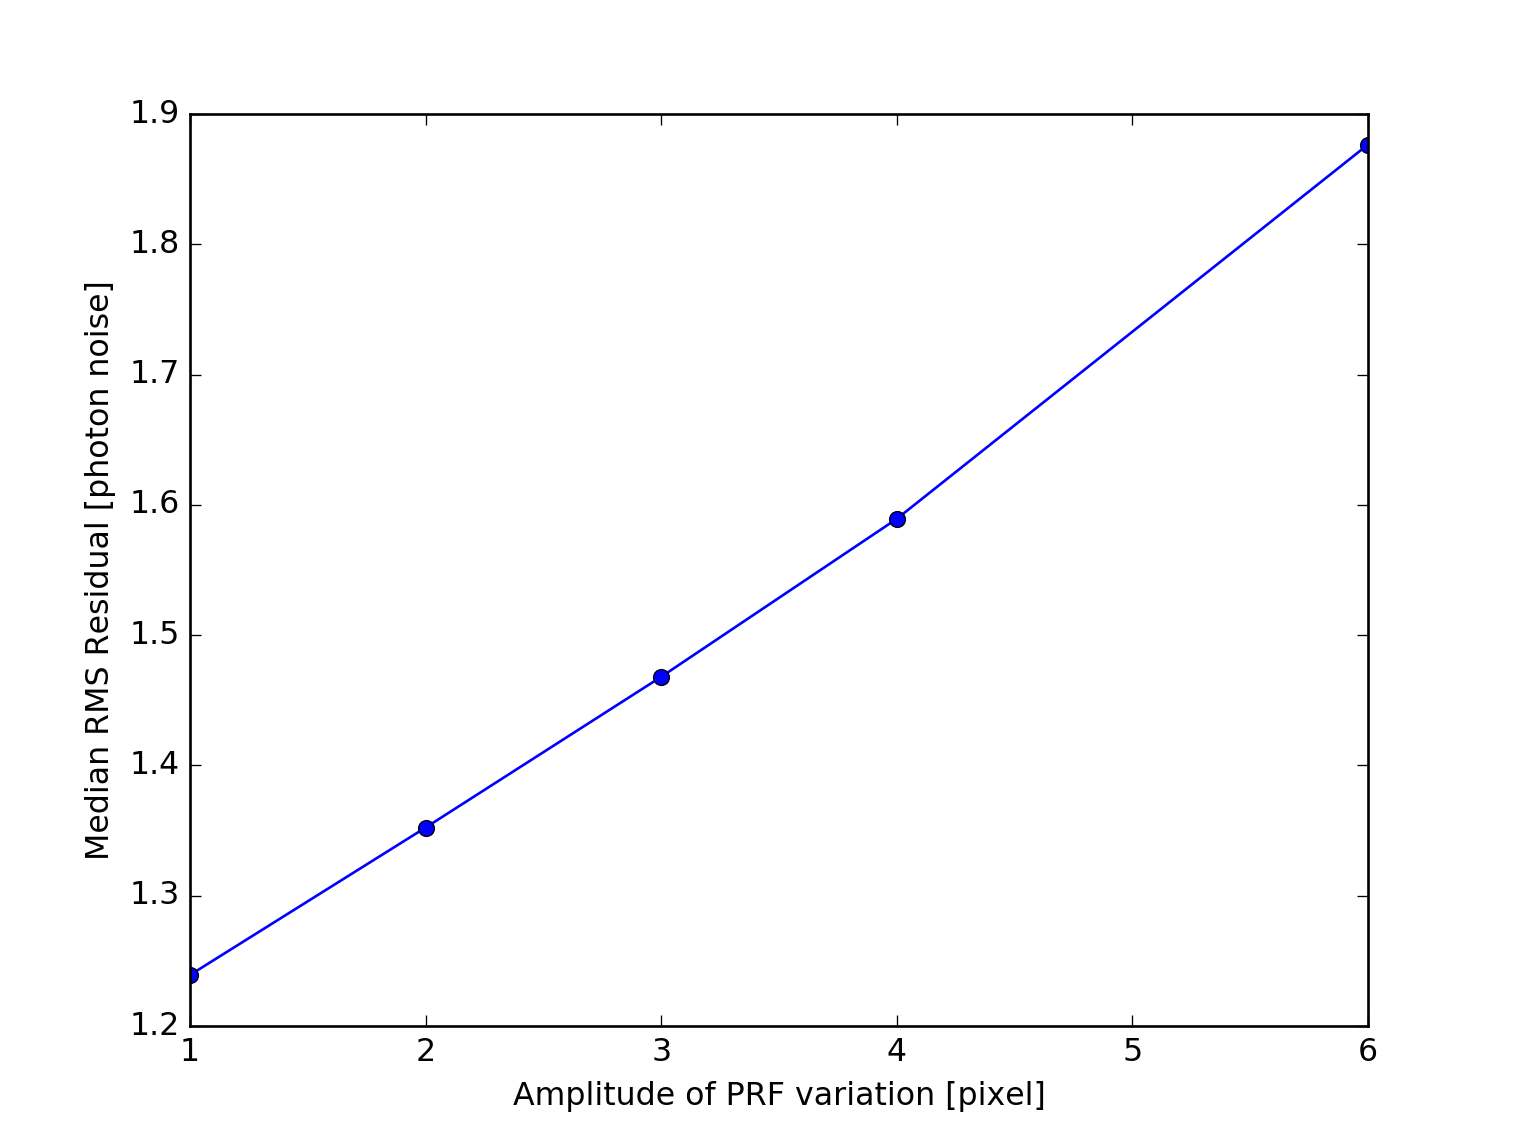
\includegraphics[width=0.95\textwidth]{prf_p}
\end{center}
\caption{
\label{prf_rms}
 Median root-mean-square residual as a function of the amplitude of PRF variation.
}
\end{figure}

\section{Discussion}
It has been demonstrated that the \cpmdiff\ is able to predict the image with precision close to the photon noise, while preserve the variable sources with both space-based and ground-based data with moderate pointing, rotation and PSF variations. 
Here we list few reasons \cpmdiff\ may be preferred over other methods:

\begin{enumerate}
\item All \class\ approachs require precise image registration as a priori step. 
Any astrometric alignment error between image frames will lead to imperfection of subtraction.
In comparison, the precision requirement of registration is largely relaxed in \cpmdiff. 
As demonstrated in Section \ref{limits}, with pointing variation smaller than $\sim$1 FWHM of PSF, precision close to photon noise can still be achieved by our method.  

\item All \class\ approcahs require direct or indirect information of the PSF. 
\cite{imagesub1}, \cite{alard} and \cite{bramich} model the difference of PSFs between images by solving the convolution kernel.
In \cite{optimal}, both PSFs of reference and new images need to be known explicitly.
Any imperfection of the PSF(or difference of PSFs) estimation will lead to subtraction residuals.
\cpmdiff\ avoids PSF estimation, since there is no convolution kernel in subtraction.

\item For photometry, de-trending process may also be required after image subtraction in the classical approach to account for extra variabilities induced by intra-and inter-pixel variations.
In comparison, \cpmdiff\ mitigates these effects internally.
\end{enumerate}

Although \cpmdiff\ performances impressively in the paper,  in order to fully exploit the potential of the method, it is still essential to find an optimal set of hyper-parameters and optimize the selection of predictors as mentioned in Section \ref{method}. 
In the original \cpm, there are two hyper-parameters---the number of predictor pixels N and the strength of the L2-regularization $\lambda_a$, which can be optimized by cross-validation. 
However, the selection or ranking of the predictor pixels are intuitively defined by either using the closest pixels in space or in brightness.
This intuitive setting is neither fully tested nor optimal, so exploring how to filter or select predictor pixels are necessary to achieve better performance of the model.
There are many ways worth trying to improve the selection of predictors.
For example, one can filter the predictor pixels by variability of the pixel.
Ideally, only quiet pixels that do not contain much variability from variable stars should be included in the predictor set, since variable predictor pixels may distort the target pixel or introduce artefacts.
Therefore if possible, all the known variable pixels should be excluded from the predictor set. 
Another way to improve can be running \cpm\ with L1-regularization and a large set of pixels. 
Since L1-regularization leads to sparsity of the coefficients, it can filter the pixels that do not contribute in the fitting. 
Other feature reduction and extraction methods such as PCA or adding higher order components might also possibly improve the set of the predictors and further enhance the performance of the model. 

To conclude, the new approach of image differencing---\cpmdiff\ is capable of variability search in time-domain imaging from both space-based and ground-based data.
The performance of the method can still be further enhanced by optimizing the hyper-parameters or exploring the possible way to improve the predictor set.
We hope \cpmdiff\ can be useful and achieve more scientific results in the future survey such as \project{LSST} and \project{TESS}.

\acknowledgements
It is a pleasure to thank
  Federica B. Bianco (NYU)
  and
  Dustin Lang (Toronto)
for valuable comments and suggestions.
This research was partially supported by
  NASA (grant NNX12AI50G),
  NSF (grants IIS-1124794, AST-1312863, AST-1517237),
  and NG Next.
The data analysis presented in this article was partially performed on computational resources at NYU HPC.
This research made use of the NASA Astrophysics Data System.


\clearpage
\bibliography{cdi}
\clearpage

\end{document}